\documentclass[a4paper,12pt]{article}
\usepackage[brazilian]{babel}
\usepackage{titlesec}
\usepackage{array}
\usepackage{indentfirst}
\titleformat*{\section}{\large\bfseries}
\usepackage{multirow}
\usepackage{hyperref}
\usepackage[lmargin=3cm,tmargin=3cm,rmargin=2cm,bmargin=2cm]{geometry}
\usepackage{iftex}
\usepackage{lipsum}
% \ifPDFTeX
%   \usepackage[activate={true,nocompatibility},final,tracking=true,kerning=true,spacing=true,factor=1100,stretch=10,shrink=10]{microtype}
% \else
%   \usepackage{microtype}
% \fi
\usepackage{caption}
\usepackage{mathptmx}
\usepackage{cancel}
\usepackage{graphbox}
% \usepackage{gensymb}
\usepackage{amsmath}
% \usepackage[utf8]{inputenc}
\usepackage{setspace}
\usepackage{float}
\usepackage{placeins}
\makeatletter
\let\c@lofdepth\relax
\makeatother
\usepackage{tocloft}
\usepackage{booktabs}
% \usepackage{subfigure}
\usepackage{amsfonts}
\usepackage{graphicx}
\usepackage{eso-pic}
\usepackage{xcolor}
\usepackage{fontspec}
\usepackage{fancyhdr}
\usepackage{listings}
\usepackage{xcolor}
\renewcommand{\cftsecleader}{\cftdotfill{\cftdotsep}}
\setlength{\cftbeforesecskip}{0.5em}
\captionsetup[figure]{labelsep= endash}


% Define Shell style for listings
\lstdefinestyle{shellstyle}{
    backgroundcolor=\color{gray!10},    % light gray background
    basicstyle=\ttfamily\small,         % monospace font, small size
    numbers=left,                       % line numbers on the left
    numberstyle=\tiny\color{gray},      % line number style
    numbersep=8pt,                     % space between line numbers and code
    frame=none,                       % no frame around the code
    rulecolor=\color{black!30},
    breaklines=true,                  % automatic line breaking
    keywordstyle=\color{blue}\bfseries,   % keywords in bold blue
    commentstyle=\color{green!50!black}\itshape, % comments in italic dark green
    stringstyle=\color{red},           % strings in red
    showstringspaces=false,            % no special string space marking
    tabsize=4,
    language=bash                   % MATLAB language support
}

\newcommand\ColocarImagemCapa{%
  \AddToShipoutPictureBG*{%
    
\includegraphics[%
      width=\paperwidth,
      height=\paperheight,
      keepaspectratio=false
    ]{imgs/gerais/capa.png}%
  }%
}

\newcommand\ColocarImagemSumario{%
  \AddToShipoutPictureBG*{%
    \includegraphics[%
      width=\paperwidth,
      height=\paperheight,
      keepaspectratio=false
    ]{imgs/gerais/sumário.png}%
  }%
}

\newcommand{\logoep}{
\includegraphics[height=1.3cm]{imgs/gerais/Logo EP.jpg}}

\newcommand{\logocurso}{
\includegraphics[height=1.3cm]{imgs/gerais/Logo Curso.jpg}}


\pagestyle{fancy}
\fancyhf{}  % Limpa os cabeçalhos e rodapés padrões
\setlength{\headheight}{1.5cm}  % Ajusta a altura do cabeçalho para acomodar a logo
\setlength{\headsep}{1.5cm}     % Ajusta o espaçamento entre o cabeçalho e o conteúdo

% Definir logo no cabeçalho à esquerda
\fancyhead[R]{\logoep}  % Coloca a logo à esquerda
\fancyhead[L]{\logocurso}


\setlength{\footskip}{1cm}  % Ajusta a altura do rodapé
\setlength{\textheight}{23cm}

\fancyfoot[C]{\textbf{\thepage}}  % Coloca o número da página no rodapé centralizado

\begin{document}

    \begin{titlepage}
\setmainfont{Arial}
\ColocarImagemCapa


    \begin{center}
        \begin{minipage}[c]{0.62\textwidth}
        \centering
            \vspace{275pt}
            \begin{huge}
            
            \textbf{Git} \\
            \end{huge}
            \textbf{Edição: 2025} \\
            \textbf{Desenvolvido por: Antônio Kipper e Bernardo Recktenvald}
            \vfill
        \end{minipage}
    \end{center}

    \newpage
    \ColocarImagemSumario
    \tableofcontents  % Sumário
    \ColocarImagemSumario
    \thispagestyle{empty} % tirar numeração
    \newpage

\end{titlepage}

    \section{Introdução Geral}

O desenvolvimento de projetos de engenharia, especialmente na área aeroespacial, envolve o trabalho com múltiplos arquivos, modelos, códigos e documentações que são constantemente atualizados e aprimorados. Nesse cenário, manter a organização, a rastreabilidade e a colaboração entre os membros de um time é um grande desafio. Para lidar com essas demandas, o uso de sistemas de \textbf{controle de versão} tornou-se indispensável, permitindo registrar alterações, restaurar versões anteriores, integrar contribuições de diferentes colaboradores e garantir a integridade do projeto.

O \textbf{Git} é atualmente a ferramenta de controle de versão mais utilizada no mundo acadêmico e industrial. Desenvolvido inicialmente por Linus Torvalds para gerenciar o código-fonte do sistema operacional Linux, o Git tornou-se um padrão na indústria de tecnologia devido à sua eficiência, flexibilidade e suporte à colaboração distribuída. Diferente de sistemas tradicionais de controle de versão, o Git permite que cada desenvolvedor possua uma cópia completa do histórico do projeto, o que aumenta a segurança, a autonomia e a velocidade no desenvolvimento.

Além disso, o Git é amplamente integrado a plataformas como \textit{GitHub}, \textit{GitLab} e \textit{Bitbucket}, que oferecem recursos adicionais para colaboração, revisão de código, gestão de tarefas e integração com ferramentas de automação. Essas plataformas são utilizadas não apenas por empresas de tecnologia, mas também por instituições acadêmicas e equipes de pesquisa, tornando o domínio do Git uma habilidade essencial para qualquer estudante ou profissional que deseja atuar em projetos modernos e colaborativos.

O objetivo central desta apostila é introduzir o Git como uma ferramenta prática e poderosa para organização, versionamento e colaboração no desenvolvimento de projetos. Ao longo do material, os leitores serão guiados por conceitos teóricos fundamentais e exemplos práticos, de forma que, ao final, estejam aptos a criar, gerenciar e compartilhar seus próprios repositórios, além de contribuir para projetos em equipe com segurança e eficiência.

\subsection{Objetivo da Apostila}

Esta apostila foi desenvolvida pela Escola Piloto de Engenharia Aeroespacial da Universidade Federal de Santa Maria com o objetivo de apresentar, de forma clara e progressiva, os fundamentos teóricos e práticos do \textbf{Git}. O material busca capacitar os leitores para:

\begin{itemize}
    \item Compreender os conceitos essenciais de controle de versão e a importância do Git no gerenciamento de projetos;
    \item Criar e manipular repositórios locais, registrando o histórico de alterações por meio de commits;
    \item Trabalhar com repositórios remotos, utilizando plataformas como GitHub e GitLab para compartilhar e integrar projetos;
    \item Aplicar técnicas de \textit{branching} e \textit{merging} para organizar fluxos de trabalho e gerenciar o desenvolvimento colaborativo;
    \item Adotar boas práticas para escrever mensagens de commit claras, organizar arquivos e estruturar projetos de forma eficiente;
    \item Desenvolver autonomia para lidar com conflitos de versão, entender fluxos de trabalho de equipes e colaborar de maneira produtiva.
\end{itemize}

Mais do que ensinar comandos e procedimentos, esta apostila busca desenvolver uma \textbf{mentalidade de versionamento}, na qual os estudantes aprendem a pensar na evolução de um projeto como um processo estruturado, seguro e colaborativo. Ao final, espera-se que os leitores tenham adquirido não apenas conhecimento técnico, mas também uma visão prática de como o Git se integra ao ciclo de desenvolvimento de sistemas e aplicações na engenharia aeroespacial.

\subsection{Público-Alvo}

Esta apostila foi elaborada especialmente para \textbf{estudantes dos primeiros semestres do curso de Engenharia Aeroespacial} da Universidade Federal de Santa Maria, mas também pode ser útil para alunos de outros cursos de engenharia, ciência da computação e áreas afins. O material parte do princípio de que o leitor está em fase inicial de contato com ferramentas de desenvolvimento e colaboração, não exigindo conhecimentos avançados de programação ou experiência prévia com controle de versão.

Para os estudantes de engenharia aeroespacial, o domínio do Git é particularmente relevante, pois a área envolve projetos multidisciplinares que integram diferentes componentes, como simulações, modelagem matemática, controle de sistemas, análise de dados e desenvolvimento de software embarcado. Projetos colaborativos, sejam eles acadêmicos, laboratoriais ou de pesquisa, tornam-se mais organizados, seguros e eficientes com o uso do Git, permitindo gerenciar versões, acompanhar o progresso e integrar contribuições de diferentes integrantes da equipe.

Além disso, aprender Git desde os primeiros semestres proporciona aos estudantes uma base sólida para enfrentar desafios futuros, seja no desenvolvimento de trabalhos acadêmicos, na execução de projetos de pesquisa, na participação em equipes de competição tecnológica ou na preparação para estágios e oportunidades no setor aeroespacial.

\subsection{Estrutura da Apostila}

A apostila foi organizada de forma progressiva, abordando desde os conceitos fundamentais até práticas mais avançadas de versionamento e colaboração. Sua estrutura é dividida em seções principais:

\begin{itemize}
    \item \textbf{Conceitos Básicos de Git:} Introdução ao controle de versão, instalação e configuração inicial.
    \item \textbf{Primeiros Passos com Git:} Criação de repositórios, rastreamento de arquivos, commits e fluxo de trabalho.
    \item \textbf{Trabalhando com Repositórios Remotos:} Integração com plataformas como GitHub, envio e atualização de projetos.
    \item \textbf{Colaboração e Trabalho em Equipe:} Revisão de código, pull requests e boas práticas de contribuição.
    \item \textbf{Branching e Merging:} Criação e gerenciamento de branches, resolução de conflitos e organização do desenvolvimento.
    \item \textbf{Boas Práticas:} Estratégias para mensagens de commit, organização de repositórios e metodologias como GitFlow.
    \item \textbf{Exercícios Práticos:} Atividades guiadas para consolidar os conhecimentos, incluindo um mini-projeto colaborativo.
    \item \textbf{Recursos e Referências:} Fontes de estudo e materiais de apoio para aprofundar o aprendizado.
\end{itemize}

Com essa abordagem, espera-se que o leitor desenvolva não apenas o domínio técnico sobre os comandos do Git, mas também a compreensão de como aplicar essas ferramentas para melhorar a organização, a produtividade e a qualidade de projetos individuais e colaborativos.

    \newpage
\section{Conceitos Básicos de Git}
\subsection{Motivação para o Controle de Versão}

Durante a graduação em Engenharia Aeroespacial, os estudantes frequentemente trabalham em projetos que envolvem diversos arquivos, como relatórios, códigos de simulação, diagramas, modelos matemáticos e documentação técnica. Esses projetos evoluem constantemente: novos recursos são adicionados, erros são corrigidos e diferentes versões dos arquivos são criadas ao longo do tempo. Em equipes, esse processo torna-se ainda mais complexo, pois várias pessoas modificam os mesmos arquivos simultaneamente.

Em um cenário sem controle de versão, os problemas aparecem rapidamente. Imagine um grupo de estudantes desenvolvendo um modelo de dinâmica orbital no \textit{MATLAB/Simulink} para uma disciplina de Mecânica Espacial. Cada integrante precisa ajustar parâmetros, modificar funções e atualizar gráficos. Sem uma ferramenta adequada, seria comum surgirem situações como:

\begin{itemize}
    \item Várias cópias do mesmo arquivo com nomes diferentes, como \texttt{simulacao\_final.m}, \texttt{simulacao\_final\_corrigida.m} ou \texttt{simulacao\_nova\_versao\_FINAL.m};
    \item Perda de trabalho por sobrescrever arquivos de colegas sem querer;
    \item Dificuldade em identificar qual versão contém os resultados corretos;
    \item Retrabalho ao tentar combinar manualmente alterações feitas por diferentes membros da equipe;
    \item Falta de histórico, tornando impossível “voltar atrás” para recuperar uma versão anterior que funcionava.
\end{itemize}

Agora, considere outro exemplo: um projeto interdisciplinar envolvendo a modelagem aerodinâmica de um veículo hipersônico. Os alunos trabalham com diversos tipos de arquivos — simulações de dinâmica de fluidos, códigos de processamento de dados, gráficos de desempenho, relatórios técnicos e apresentações. Sem um sistema organizado, fica praticamente impossível coordenar todas as contribuições, documentar mudanças e garantir que os resultados sejam confiáveis.

É nesse contexto que entra o \textbf{Git}, um sistema de \textit{controle de versão distribuído} que permite:

\begin{itemize}
    \item Registrar todas as alterações realizadas no projeto, criando um histórico completo e detalhado;
    \item Criar diferentes versões dos arquivos sem precisar duplicá-los;
    \item Trabalhar de forma colaborativa, permitindo que várias pessoas editem o mesmo projeto simultaneamente;
    \item Integrar mudanças de forma controlada, evitando conflitos e perdas de dados;
    \item Retornar facilmente para versões anteriores, caso seja necessário corrigir erros ou recuperar resultados antigos.
\end{itemize}

O Git funciona como uma \textbf{“linha do tempo”} do projeto. Cada modificação feita nos arquivos pode ser registrada em um \textit{commit}, criando um ponto de restauração com informações sobre quem alterou, quando alterou e por quê. Isso é especialmente útil em trabalhos acadêmicos e projetos colaborativos, pois permite que todos acompanhem o histórico e a evolução dos resultados.

Além disso, quando combinado com plataformas como o \textit{GitHub} e o \textit{GitLab}, o Git potencializa a colaboração entre equipes, permitindo que os integrantes compartilhem seus projetos, revisem código, comentem alterações e integrem contribuições de forma organizada. Para estudantes de Engenharia Aeroespacial, isso significa maior eficiência no desenvolvimento de simulações, controle de modelos complexos e integração de dados experimentais.

Em resumo, o Git não é apenas uma ferramenta para desenvolvedores de software: ele é um aliado fundamental no gerenciamento de projetos de engenharia. Ele garante organização, segurança, rastreabilidade e colaboração, preparando os estudantes para lidar com desafios acadêmicos e profissionais, tanto na universidade quanto na indústria aeroespacial.

\subsection{O que é Git}

O \textbf{Git} é um \textit{sistema de controle de versão distribuído} desenvolvido por Linus Torvalds em 2005 para gerenciar o código-fonte do sistema operacional Linux. Em termos simples, o Git permite registrar, organizar e acompanhar todas as alterações realizadas em um conjunto de arquivos, garantindo segurança, rastreabilidade e eficiência no desenvolvimento de projetos.

Em vez de criar várias cópias de um mesmo arquivo com nomes diferentes, como \texttt{simulacao\_final.m} ou \texttt{relatorio\_versao2.docx}, o Git mantém um \textbf{histórico detalhado} de tudo o que foi modificado, quem fez a alteração, quando e por quê. Cada modificação é registrada por meio de um \textit{commit}, que funciona como um “ponto de controle” na linha do tempo do projeto. Isso permite que você volte para versões anteriores a qualquer momento, sem perder dados.

Para estudantes de Engenharia Aeroespacial, isso é particularmente útil. Imagine um projeto de simulação de voo atmosférico desenvolvido no \textit{MATLAB/Simulink}. Durante o semestre, vários ajustes são realizados: mudanças nos parâmetros de altitude, novas funções para modelar a resistência do ar e gráficos para analisar a estabilidade da trajetória. Sem Git, seria necessário salvar manualmente várias versões dos arquivos para evitar perder o progresso. Com o Git, basta registrar as alterações e, se necessário, restaurar qualquer estado anterior do projeto com um único comando.

Outro benefício do Git é que ele é \textbf{distribuído}: cada membro de uma equipe tem uma cópia completa do repositório, incluindo todo o histórico do projeto. Isso significa que o trabalho não depende de um servidor central — você pode continuar desenvolvendo mesmo sem conexão com a internet e sincronizar suas alterações mais tarde. Essa característica é valiosa para projetos colaborativos, como laboratórios, trabalhos em grupo e competições acadêmicas, onde diferentes integrantes contribuem simultaneamente para o mesmo código, modelo ou relatório.

Em resumo, o Git é mais do que uma ferramenta para programadores: ele é um recurso essencial para organizar, versionar e colaborar em projetos complexos, garantindo que todas as etapas do desenvolvimento sejam registradas e facilmente acessíveis.

\subsection{Git vs GitHub vs GitLab}

É comum confundir o \textbf{Git} com plataformas como \textbf{GitHub} e \textbf{GitLab}, mas há uma diferença importante entre eles:

\begin{itemize}
    \item \textbf{Git} — É a \textbf{ferramenta} de controle de versão em si. Ela roda no seu computador e permite criar repositórios, registrar alterações, criar branches, fazer merges e gerenciar o histórico do projeto. Você pode usar o Git localmente, sem precisar estar conectado à internet.

    \item \textbf{GitHub} — É uma \textbf{plataforma online} que hospeda repositórios Git e oferece recursos extras para colaboração, como revisão de código, gerenciamento de tarefas, abertura de \textit{issues} e integração com ferramentas externas. É amplamente utilizada no meio acadêmico e industrial para armazenar projetos abertos e privados. Além disso, o GitHub facilita o compartilhamento de trabalhos com professores, colegas e equipes de pesquisa.

    \item \textbf{GitLab} — Também é uma \textbf{plataforma online} para hospedagem de repositórios Git, semelhante ao GitHub, mas com foco maior em integração contínua, automação de testes e gestão de projetos. Muitas empresas e instituições de pesquisa preferem o GitLab por permitir a instalação de servidores privados, garantindo maior controle sobre os dados e a segurança dos projetos.
\end{itemize}

Um exemplo prático: imagine que um grupo de estudantes de Engenharia Aeroespacial está desenvolvendo um \textbf{simulador de trajetória de foguetes} para um projeto interdisciplinar. O \textbf{Git} seria utilizado para gerenciar o histórico do código e das simulações localmente. Para colaborar com os colegas, compartilhar resultados e revisar contribuições, o grupo poderia criar um repositório remoto no \textbf{GitHub} ou no \textbf{GitLab}, permitindo que todos sincronizem suas alterações com facilidade. Caso o projeto fosse confidencial ou envolvesse dados sensíveis, o \textbf{GitLab} poderia ser configurado em um servidor interno da instituição, oferecendo mais privacidade e controle.

Em resumo:
\begin{itemize}
    \item \textbf{Git} = ferramenta de controle de versão local.
    \item \textbf{GitHub/GitLab} = plataformas que usam o Git para facilitar colaboração, hospedagem e integração.
\end{itemize}

Na prática, você usará o Git para versionar e gerenciar seus arquivos, e o GitHub ou GitLab para compartilhar o projeto e trabalhar de forma colaborativa com sua equipe.

\subsection{Instalação e Configuração Inicial do Git}

Antes de começarmos a utilizar o Git, é necessário instalá-lo e preparar o ambiente de desenvolvimento. O processo de instalação varia de acordo com o sistema operacional, mas o objetivo final é o mesmo: permitir que você crie e gerencie repositórios locais e trabalhe com plataformas remotas, como GitHub e GitLab.

Nesta apostila, recomendamos também o uso do \textbf{Visual Studio Code (VS Code)} como editor de código. Ele é gratuito, multiplataforma e possui integração nativa com o Git, permitindo visualizar alterações, realizar commits, gerenciar branches e sincronizar repositórios diretamente.

A seguir, apresentamos os passos para instalação no macOS, Linux e Windows.

\subsubsection*{Instalação no macOS}

\begin{enumerate}
    \item \textbf{Verificar se o Git já está instalado}  
    Abra o \textit{Terminal} e execute:
    \begin{lstlisting}[style=shellstyle]
 git --version
    \end{lstlisting}
    Se o Git já estiver instalado, o comando exibirá a versão atual. Caso contrário, siga os próximos passos.

    \item \textbf{Instalar o Git usando o Homebrew (recomendado)}  
    Primeiro, instale o Homebrew:
    \begin{lstlisting}[style=shellstyle]
/bin/bash -c "$(curl -fsSL https://raw.githubusercontent.com/Homebrew/install/HEAD/install.sh)"
    \end{lstlisting}
    Em seguida, instale o Git:
    \begin{lstlisting}[style=shellstyle]
brew install git
    \end{lstlisting}

    \item \textbf{Instalar o Visual Studio Code}  
    Acesse o site oficial:  
    \url{https://code.visualstudio.com/}  
    Baixe a versão para macOS e siga as instruções de instalação.
\end{enumerate}

\subsubsection*{Instalação no Linux (Ubuntu/Debian)}

\begin{enumerate}
    \item \textbf{Verificar se o Git já está instalado}  
    Abra o \textit{Terminal} e execute:
    \begin{lstlisting}[style=shellstyle]
git --version
    \end{lstlisting}
    Caso não esteja instalado, prossiga com os próximos passos.

    \item \textbf{Instalar o Git via gerenciador de pacotes}  
    Para distribuições baseadas em Debian/Ubuntu:
    \begin{lstlisting}[style=shellstyle]
sudo apt update
sudo apt install git
    \end{lstlisting}
    Para distribuições baseadas em Fedora/RHEL:
    \begin{lstlisting}[style=shellstyle]
sudo dnf install git
    \end{lstlisting}

    \item \textbf{Instalar o Visual Studio Code}  
    Baixe o pacote \texttt{.deb} (para Ubuntu/Debian) ou \texttt{.rpm} (para Fedora) no site oficial:  
    \url{https://code.visualstudio.com/}  

    Alternativamente, no Ubuntu/Debian, você pode instalar via terminal:
    \begin{lstlisting}[style=shellstyle]
sudo snap install code --classic
    \end{lstlisting}
\end{enumerate}

\subsubsection*{Instalação no Windows}

\begin{enumerate}
    \item \textbf{Baixar o instalador do Git}  
    Acesse o site oficial:  
    \url{https://git-scm.com/download/win}  
    Faça o download do instalador mais recente.

    \item \textbf{Executar o instalador}  
    Durante a instalação, mantenha as opções padrão recomendadas, especialmente:
    \begin{itemize}
        \item Instalar o \textbf{Git Bash} — um terminal otimizado para comandos Git.
        \item Configurar o editor padrão como \textbf{Visual Studio Code}, caso já esteja instalado.
    \end{itemize}

    \item \textbf{Instalar o Visual Studio Code}  
    Caso ainda não tenha o VS Code, baixe-o no site oficial:  
    \url{https://code.visualstudio.com/}  
    Durante a instalação, marque a opção \textit{"Add to PATH"} para facilitar a integração com o Git.
\end{enumerate}

\subsubsection*{Configuração Inicial do Git (para todos os sistemas)}

Após instalar o Git, é necessário configurá-lo pela primeira vez. Essas configurações são feitas uma única vez e serão aplicadas a todos os seus repositórios no computador.

\begin{enumerate}
    \item \textbf{Definir nome e e-mail}  
    Esses dados serão utilizados para identificar quem realizou cada alteração no projeto:
    \begin{lstlisting}[style=shellstyle]
git config --global user.name "Seu Nome"
git config --global user.email "seu.email@exemplo.com"
    \end{lstlisting}

    \item \textbf{Verificar as configurações}  
    Para confirmar se as credenciais foram registradas corretamente:
    \begin{lstlisting}[style=shellstyle]
git config --list
    \end{lstlisting}
\end{enumerate}

Após concluir esses passos, o ambiente estará pronto para criar repositórios, versionar arquivos e integrar seus projetos com plataformas como GitHub e GitLab.


\subsection{Como Registrar-se no GitHub}

% ber - colocar imagens no passo a passo do github

Para começar a utilizar o GitHub e aproveitar todos os recursos de colaboração, siga este passo a passo detalhado para criar sua conta:

\begin{enumerate}
    \item \textbf{Acesse o site oficial:}  
    Abra o navegador e digite \url{https://github.com/}.

    \item \textbf{Clique em "Sign up":}  
    No canto superior direito da página inicial, clique no botão \textbf{Sign up} para iniciar o processo de registro, como mostrado na Figura \ref{fig:sign_up}.

    \begin{figure}[H]
\centering
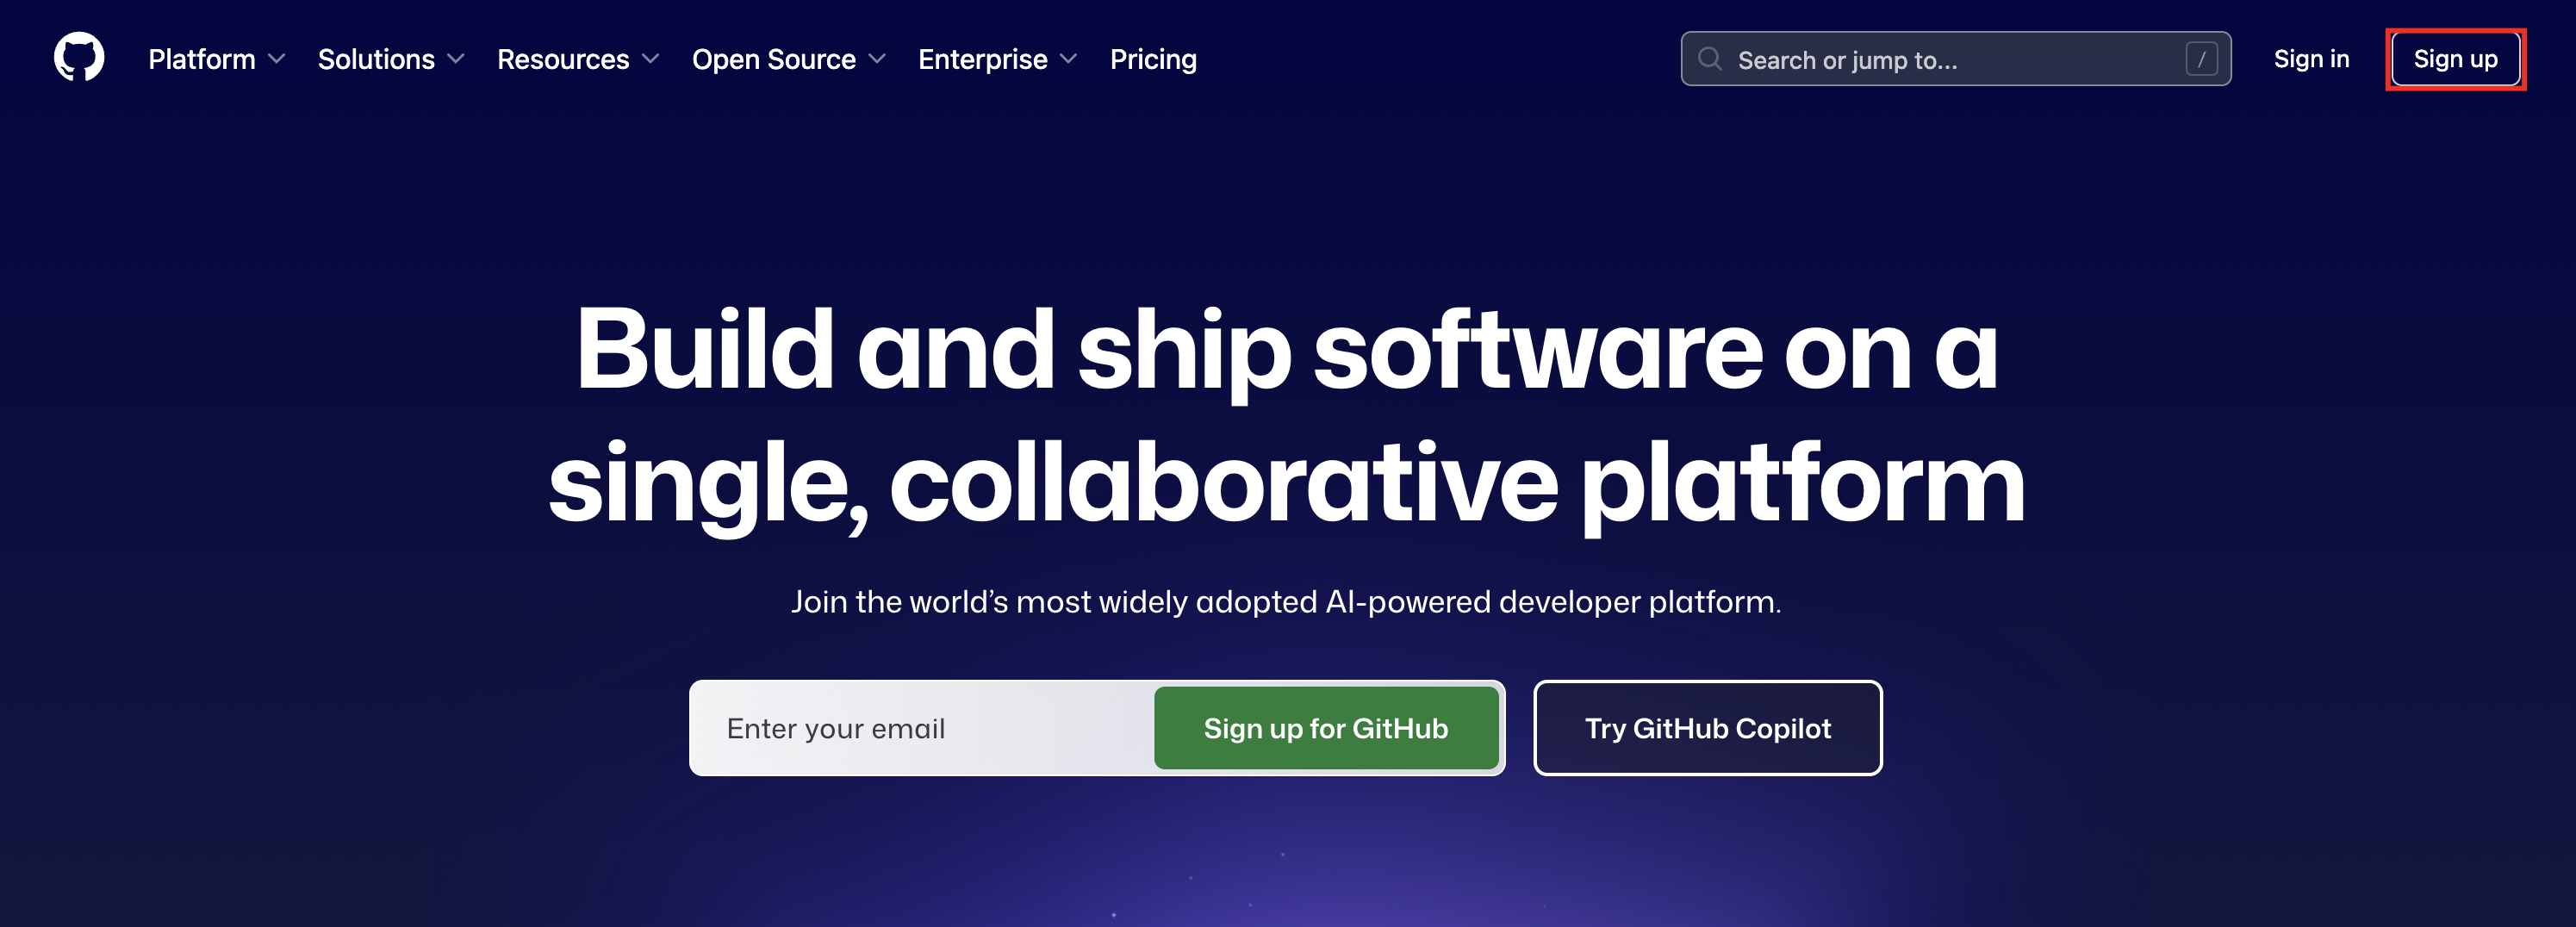
\includegraphics[width=0.6\textwidth]{imgs/tutorial_criar_conta_github/1_sign_up.png}
\caption{Botão "Sign up".}
\label{fig:sign_up}
\end{figure}

    \item \textbf{Informe seu e-mail, nome de usuário desejado e senha e crie sua conta.}  
    Digite um endereço de e-mail válido. Você receberá um código de verificação neste e-mail. Escolha um nome de usuário único, que será seu identificador público no GitHub. Crie uma senha forte. Clique no botão "Create account" para continuar, como mostrado na Figura \ref{fig:create_account}.
    
\begin{figure}[H]
\centering
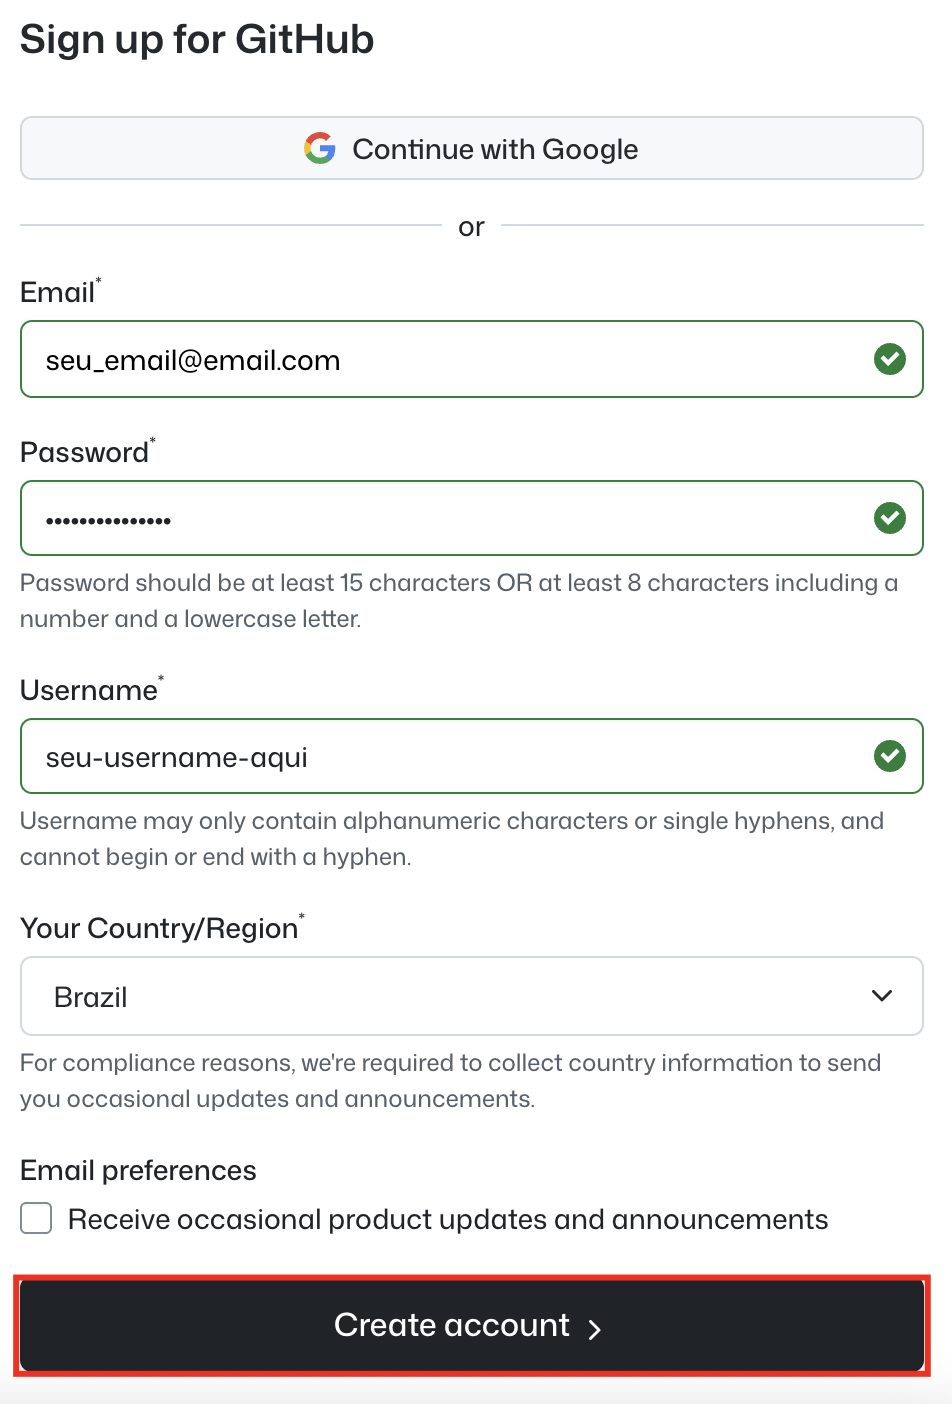
\includegraphics[width=0.5\textwidth]{imgs/tutorial_criar_conta_github/2_create_account.png}
\caption{Informações da conta e botão "Create account".}
\label{fig:create_account}
\end{figure}


    \item \textbf{Informe o código enviado ao e-mail.}  
    Caso necessário, informe o código enviado ao seu e-mail.

    \item \textbf{Configuração inicial:}  
    Após o cadastro e primeira conexão na sua conta, você pode adicionar uma foto de perfil, preencher sua bio e configurar autenticação em dois fatores para maior segurança. Para isso, primeiro clique na sua foto de perfil, no canto direito superior da página inicial, como mostrado na Figura \ref{fig:profile_image}.

\begin{figure}[H]
\centering
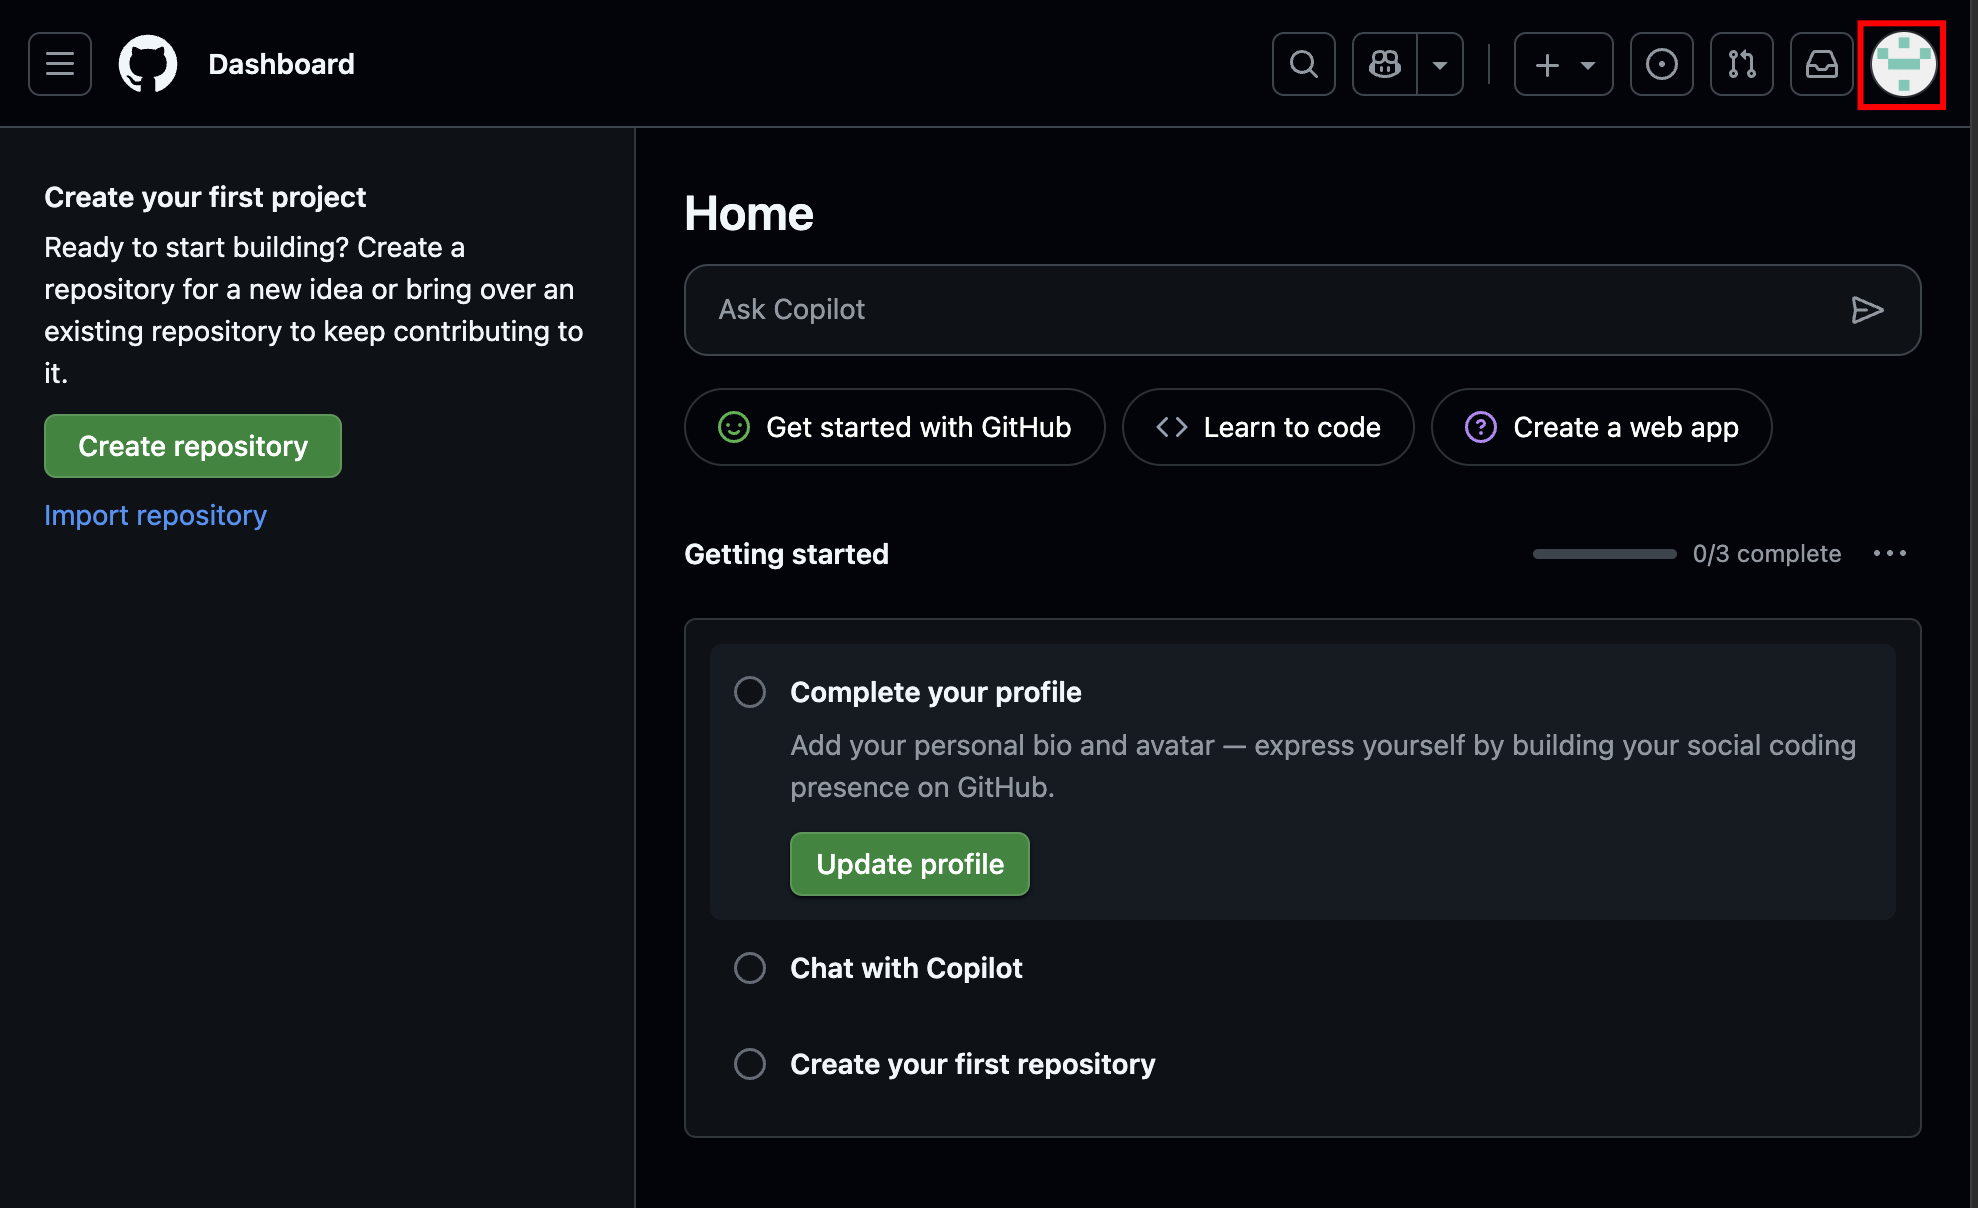
\includegraphics[width=0.6\textwidth]{imgs/tutorial_criar_conta_github/3_profile_image.png}
\caption{Foto de perfil no Github.}
\label{fig:profile_image}
\end{figure}

    \item \textbf{Navegue até as configurações do perfil:}
    Clique na aba "Profile", como mostrado na Figura \ref{fig:profile}. 
    
\begin{figure}[H]
\centering
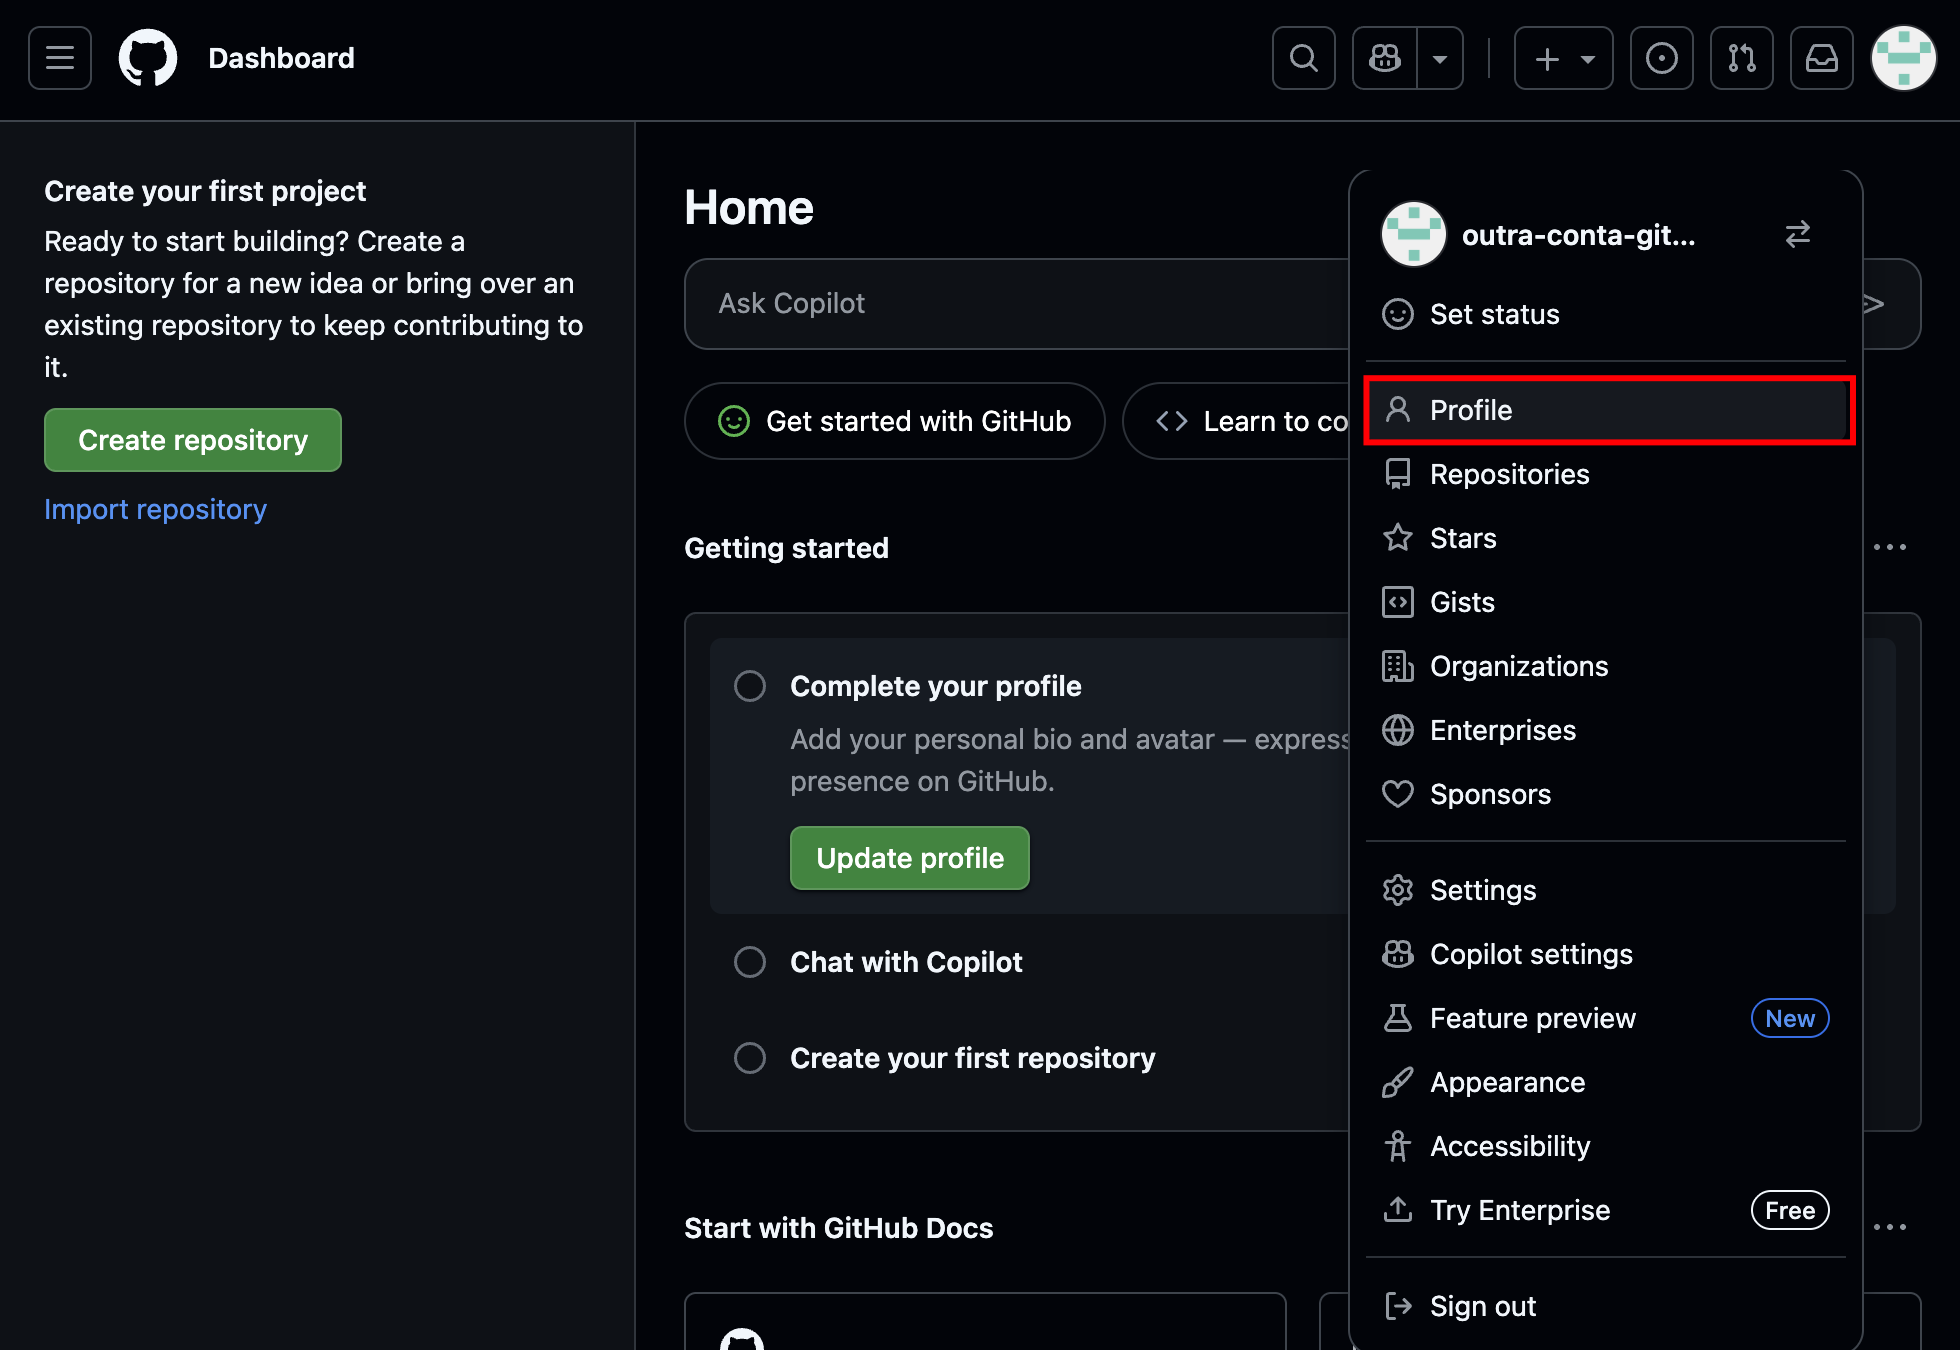
\includegraphics[width=0.6\textwidth]{imgs/tutorial_criar_conta_github/4_profile.png}
\caption{Aba "Profile" no Github.}
\label{fig:profile}
\end{figure}

Na sequência, clique em "Edit profile", como mostrado na Figura \ref{fig:edit_profile}. 

    \begin{figure}[H]
\centering
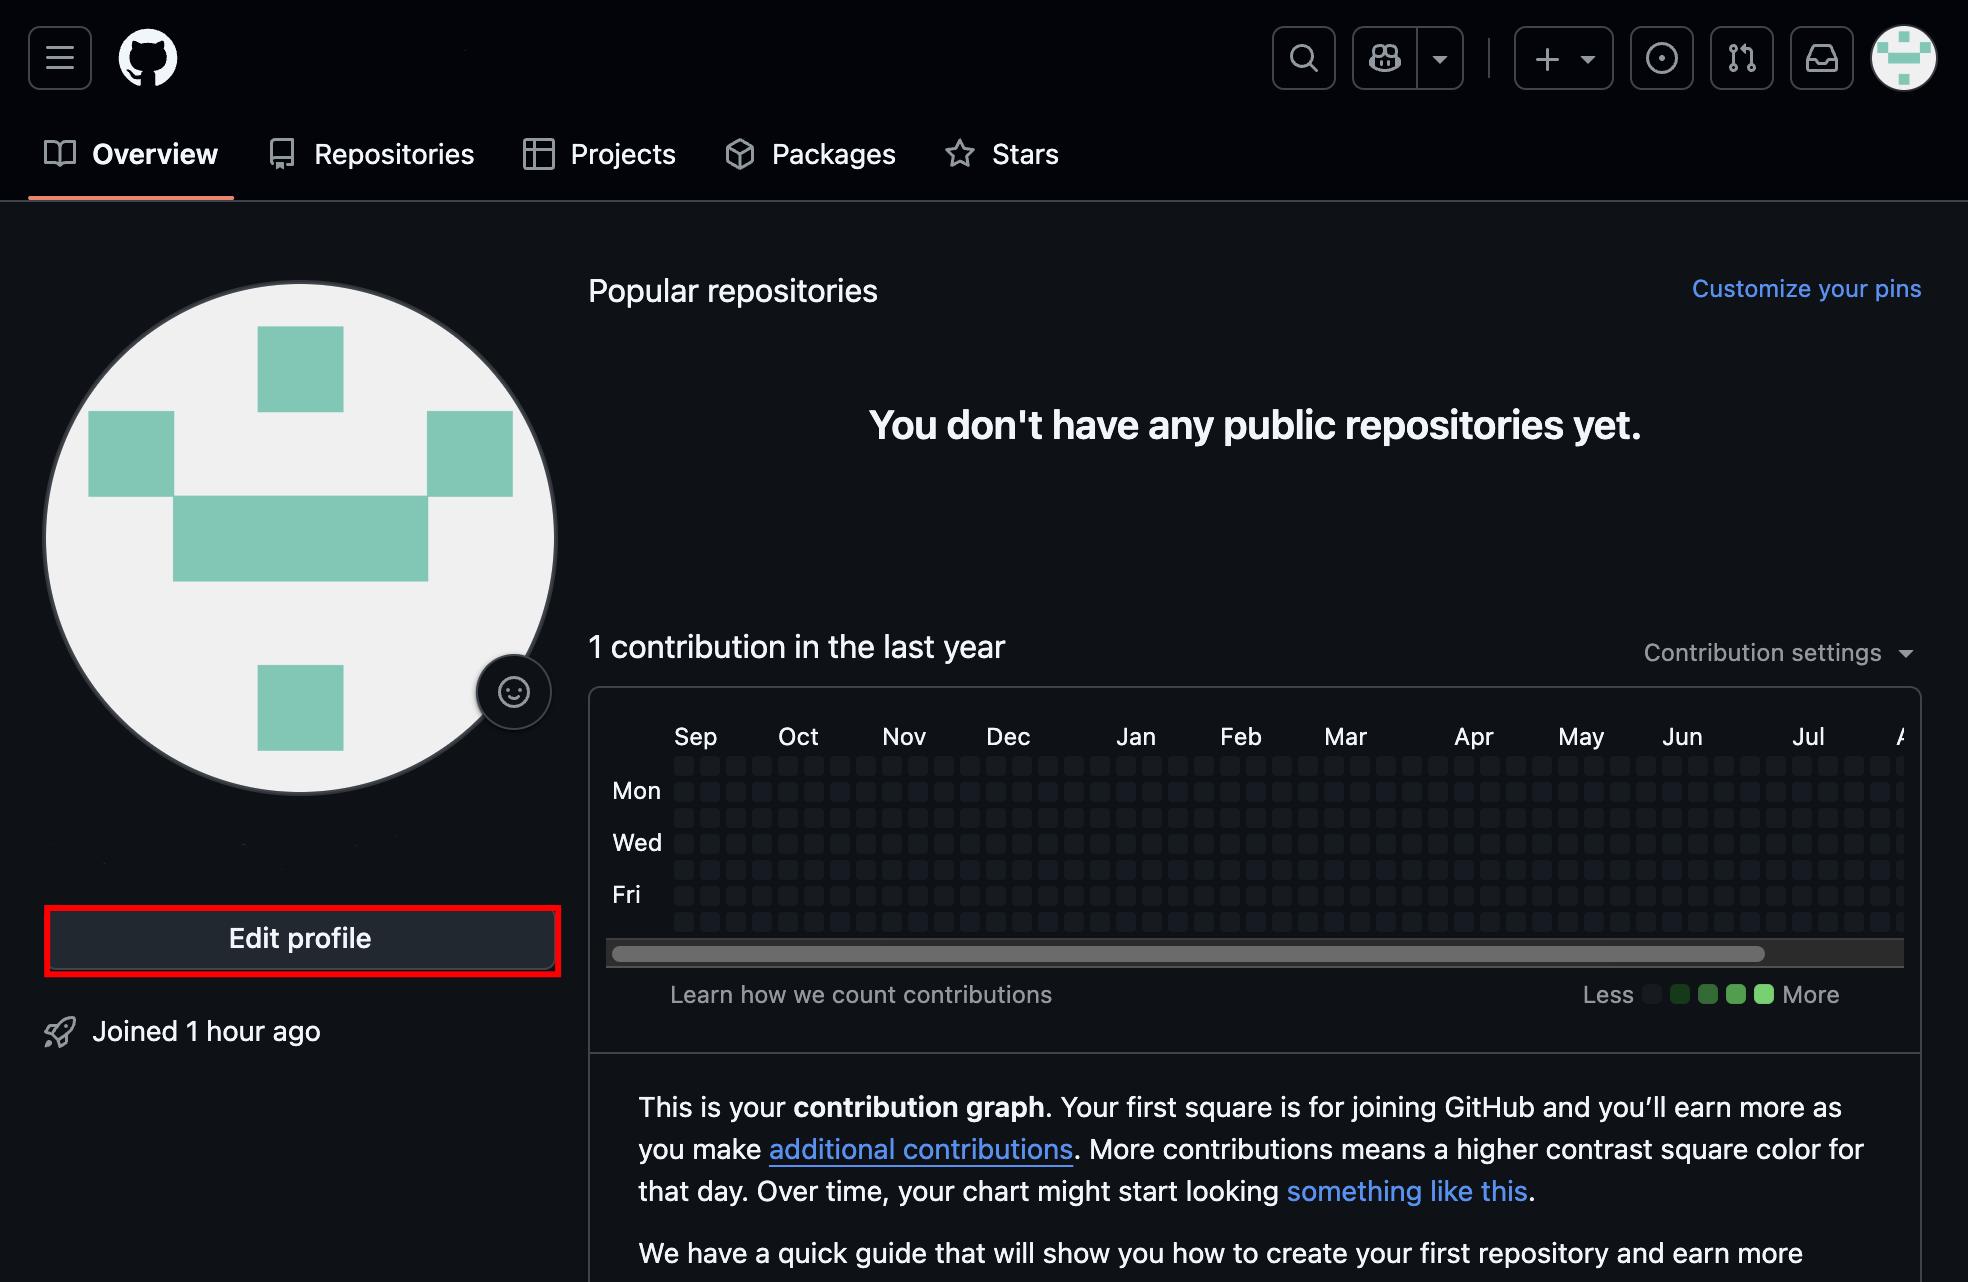
\includegraphics[width=0.6\textwidth]{imgs/tutorial_criar_conta_github/5_edit_profile.png}
\caption{Botão "Edit profile" no Github.}
\label{fig:edit_profile}
\end{figure}

Em seguida, edite as informações do seu perfil da maneira como desejar.

    \begin{figure}[H]
\centering
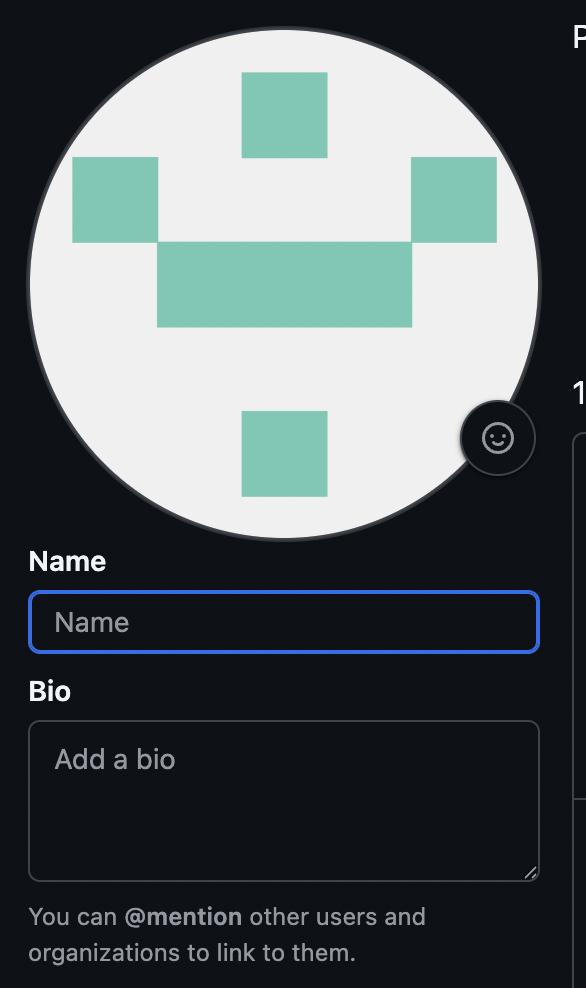
\includegraphics[width=0.4\textwidth]{imgs/tutorial_criar_conta_github/6_edit_info.png}
\caption{Configuração do seu perfil no Github.}
\label{fig:edit_info}
\end{figure}

\end{enumerate}

\subsection{Criação de uma chave SSH}
\label{cap:criacao_chave_ssh}

Para trabalhar com o GitHub, é possível realizar a comunicação com a plataforma de duas formas principais: HTTPS ou SSH.

A utilização de HTTPS é mais simples, pois não exige configuração inicial. No entanto, toda vez que for comunicar com o GitHub, é necessário informar usuário e senha ou um token de acesso.

Já o uso de SSH permite uma conexão mais prática e segura. Ao gerar uma chave SSH e adicioná-la à sua conta do GitHub, a autenticação passa a ser feita de forma automática, sem a necessidade de informar usuário e senha a cada comunicação. Essa abordagem é recomendada para quem utiliza o Git com frequência, pois agiliza o fluxo de trabalho e aumenta a segurança da comunicação.

Cada computador que se comunica com o GitHub precisa ter sua própria chave SSH. A chave é formada por duas partes: uma chave privada, que fica no computador e nunca deve ser compartilhada, e uma chave pública, que é adicionada à conta do GitHub. Assim, o GitHub reconhece o computador como autorizado a acessar os repositórios, sem precisar digitar usuário e senha a cada comunicação.

Para gerar uma chave SSH, no VS Code, abra o terminal integrado (\texttt{Ctrl + \`}) e siga os passos abaixo para gerar a chave SSH:

\begin{enumerate}
    \item Digite o comando abaixo, substituindo seu e-mail pelo utilizado no GitHub:
    \begin{lstlisting}[style=shellstyle]
ssh-keygen -t ed25519 -C "seu-email@exemplo.com"
    \end{lstlisting}
    \item Pressione \texttt{Enter} para aceitar o local padrão onde a chave será salva.
    \item Opcionalmente, digite uma senha para proteger a chave privada ou pressione \texttt{Enter} para deixar em branco.
    \item A chave será criada em duas partes: a chave privada (\texttt{id\_ed25519}) e a chave pública (\texttt{id\_ed25519.pub}).
\end{enumerate}

A chave privada deve permanecer no computador e nunca ser compartilhada. A chave pública será usada para configurar o acesso ao GitHub.

Para adicionar sua chave pública ao Github, primeiramente, copie os conteúdos do arquivo \texttt{id\_ed25519.pub}. Para fazer isso, use:

\begin{lstlisting}[style=shellstyle]
cat ~/.ssh/id_ed25519.pub
\end{lstlisting}

O comando \texttt{cat} mostra no terminal os conteúdos de um arquivo. Copie a chave mostrada. Ela deve ter o seguinte formato:

\begin{lstlisting}[style=shellstyle]
ssh-ed25519 <caracteres-aleatórios> seu-email@exemplo.com
\end{lstlisting}

Na sequência, siga os seguintes passos:

\begin{itemize}
    \item \textbf{Clique novamente na sua foto de perfil no Github:}
    Desta vez, clique na aba "Settings".

\begin{figure}[H]
\centering
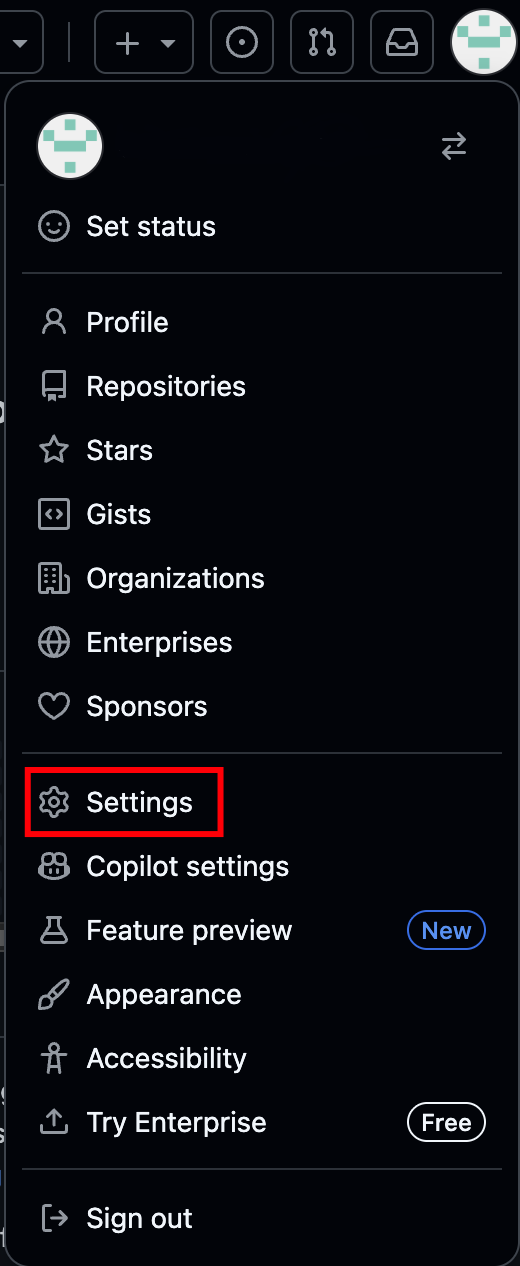
\includegraphics[width=0.3\textwidth]{imgs/tutorial_criar_conta_github/7_settings.png}
\label{fig:edit_info}
\caption{Aba "Settings" no Github.}
\end{figure}

\item \textbf{Clique na opção "SSH and GPG keys":}
Essa seção permite de configurar as chaves de acesso adicionados ao seu Github.

\begin{figure}[H]
\centering
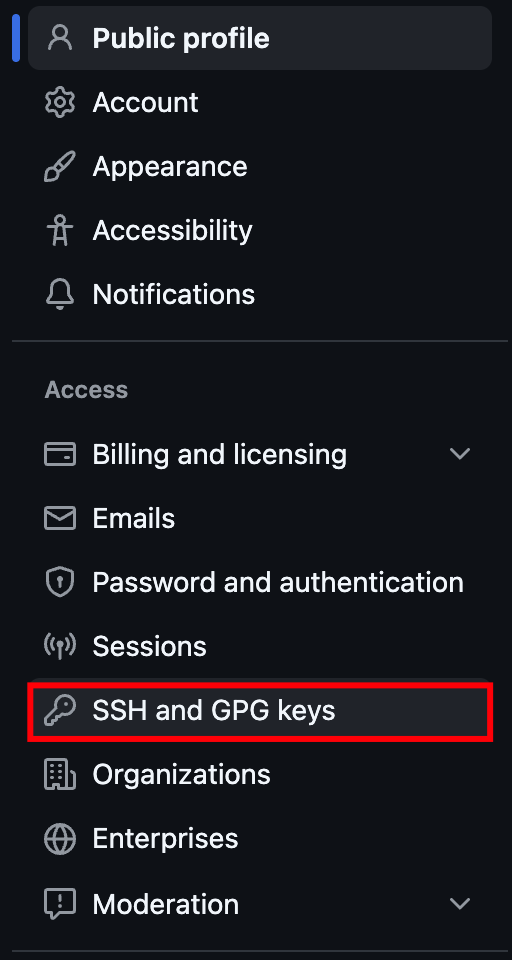
\includegraphics[width=0.4\textwidth]{imgs/tutorial_criar_conta_github/8_ssh_keys.png}
\label{fig:ssh_keys}
\caption{Opção "SSH and GPG keys".}
\end{figure}

\item \textbf{Clique em "New SSH key":}
Clique nesse botão para adicionar uma nova chave SSH.

    \begin{figure}[H]
\centering
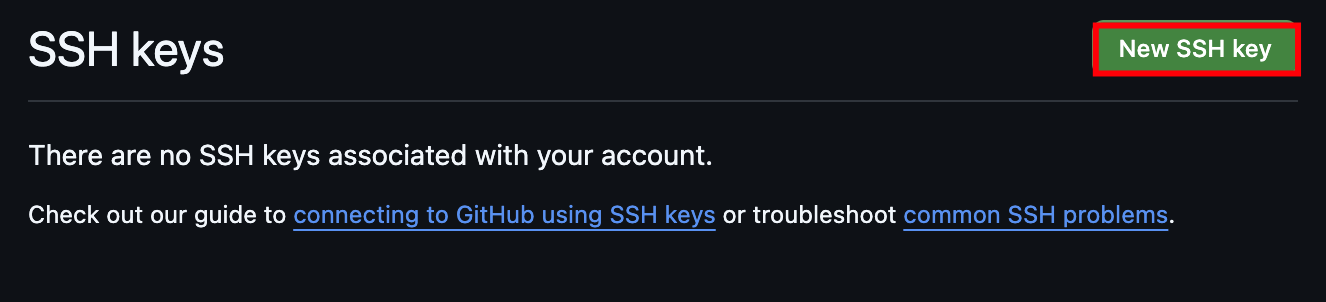
\includegraphics[width=0.8\textwidth]{imgs/tutorial_criar_conta_github/9_new_ssh_key.png}
\label{fig:ssh_keys}
\caption{Botão "New SSH key".}
\end{figure}

\item \textbf{Adicione as informações:}
    Coloque um nome que identifique a chave SSH que você está adicionando. Lembre-se que uma chave de acesso por computador é necessária. Nomes descritivos são úteis, como "Laptop" ou "Computador de casa". Cole a sua chave SSH pública. Clique em "Add SSH key" para adicionar a chave.

    \begin{figure}[H]
\centering
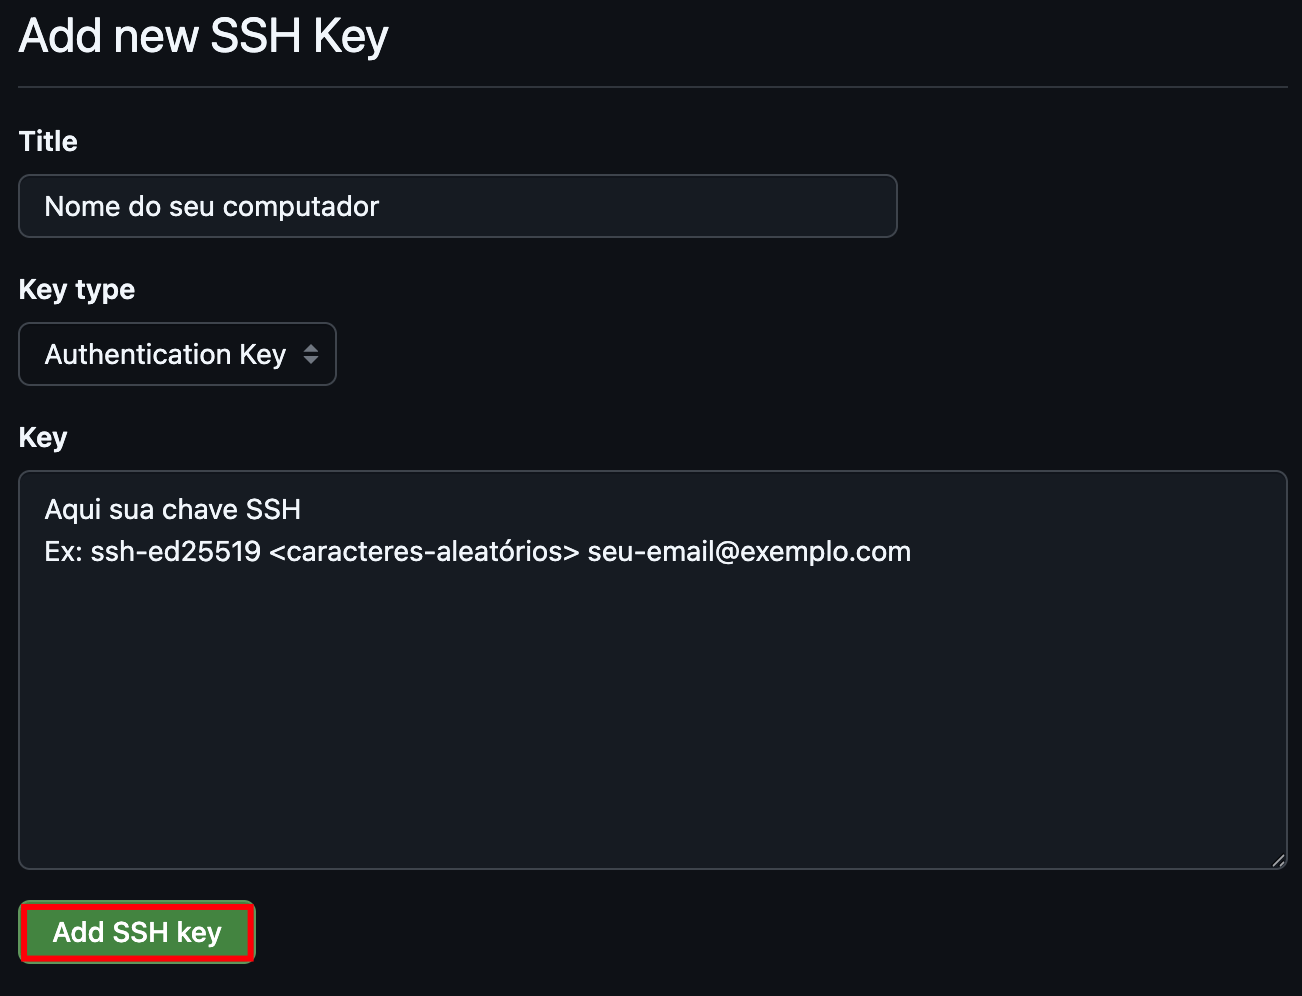
\includegraphics[width=0.5\textwidth]{imgs/tutorial_criar_conta_github/10_add_ssh_key.png}
\label{fig:ssh_keys}
\caption{Botão "Add SSH key".}
\end{figure}

\end{itemize}





    \newpage
\section{Primeiros Passos com Git}
\subsection{Criando seu Primeiro Repositório}

Um repositório é o local onde o Git armazena todo o histórico de alterações de um projeto. Ele pode ser local (no seu computador) ou remoto (em plataformas como GitHub ou GitLab). Criar seu primeiro repositório é o passo inicial para começar a versionar arquivos e acompanhar a evolução de seus projetos.

Para estudantes de Engenharia Aeroespacial, um exemplo típico seria um projeto de simulação de voo, com arquivos MATLAB/Simulink, planilhas de dados e relatórios técnicos. Ao criar um repositório, todas essas informações podem ser organizadas, versionadas e recuperadas facilmente.

\subsubsection*{Passo a Passo: Criando um Repositório Local}

1. \textbf{Escolha ou crie uma pasta para seu projeto}  
   Por exemplo, crie uma pasta chamada \texttt{simulacao\_orbital} no seu computador.

2. \textbf{Abra o terminal}  
   - No macOS ou Linux, use o Terminal.  
   - No Windows, abra o Git Bash.  
   - Alternativamente, você pode usar o terminal integrado do Visual Studio Code.

3. \textbf{Navegue até a pasta do projeto}


\begin{lstlisting}[style=shellstyle]
cd /caminho/para/simulacao_orbital
\end{lstlisting}


\textit{Comentário: O comando \texttt{cd} significa "change directory" e serve para trocar o diretório de trabalho atual no terminal. Assim, você garante que os próximos comandos do Git serão aplicados à pasta correta.}

4. \textbf{Inicialize o repositório Git}  
   Esse comando cria um repositório Git local na pasta atual, gerando a pasta oculta \texttt{.git} que armazenará o histórico do projeto:
\begin{lstlisting}[style=shellstyle]
git init
\end{lstlisting}

5. \textbf{Verifique se o repositório foi criado}  
   Execute:
\begin{lstlisting}[style=shellstyle]
git status
\end{lstlisting}
O Git mostrará que você está em um repositório vazio e pronto para adicionar arquivos.


\subsection{Rastreando Arquivos}

Após criar seu repositório, o próximo passo é informar ao Git quais arquivos você deseja versionar. Esse processo é chamado de staging, ou preparação, e é realizado com o comando \texttt{git add}. Ele permite que você escolha exatamente quais alterações serão incluídas no próximo commit.

\subsubsection*{Adicionando arquivos ao repositório}

Para adicionar todos os arquivos da pasta do projeto, execute:

\begin{lstlisting}[style=shellstyle]
git add .
\end{lstlisting}

\noindent
O ponto (\texttt{.}) indica que todos os arquivos e subpastas do diretório atual serão rastreados.  

Se você quiser adicionar apenas arquivos específicos, use:

\begin{lstlisting}[style=shellstyle]
git add simulacao.m relatorio.pdf
\end{lstlisting}

\subsubsection*{Ignorando arquivos desnecessários}

Em projetos de engenharia aeroespacial, é comum gerar arquivos temporários ou grandes que não precisam ser versionados, como:  
- Logs de simulação (\texttt{*.log})  
- Arquivos de saída do Simulink (\texttt{*.slx~})  
- Dados intermediários ou temporários (\texttt{*.mat}, \texttt{*.tmp})

Para evitar que esses arquivos sejam rastreados, crie um arquivo chamado \texttt{.gitignore} na raiz do projeto e adicione as regras:

\begin{lstlisting}[style=shellstyle]
*.log
*.slx~
*.tmp
*.mat
\end{lstlisting}

Dessa forma, o Git ignorará automaticamente esses arquivos ao executar \texttt{git add}.

\subsection{Fazendo seu Primeiro Commit}

Depois de adicionar os arquivos desejados à área de staging, o próximo passo é registrar essas alterações no repositório através de um commit. Um commit funciona como um “ponto de restauração” no histórico do projeto, permitindo recuperar versões anteriores a qualquer momento.

\subsubsection*{Criando um commit}

Para fazer o primeiro commit, execute:

\begin{lstlisting}[style=shellstyle]
git commit -m "Primeiro commit: estrutura inicial do projeto"
\end{lstlisting}

\noindent
A opção \texttt{-m} permite adicionar uma mensagem descritiva para o commit. Mensagens claras ajudam você e sua equipe a entender rapidamente o que foi alterado em cada commit.

\subsubsection*{Verificando o commit}

Após o commit, você pode conferir o histórico do repositório:

\begin{lstlisting}[style=shellstyle]
git log
\end{lstlisting}

O Git exibirá informações como:
\begin{itemize}
    \item Identificador único do commit (hash)  
    \item Autor do commit  
    \item Data e hora do commit  
    \item Mensagem do commit
\end{itemize}
    \newpage
\section{Trabalhando com Repositórios Remotos}
\subsection{Conectando-se ao GitHub}

O GitHub é uma plataforma de hospedagem de repositórios Git remotos que permite armazenar, compartilhar e colaborar em projetos. Para enviar e receber alterações de um repositório remoto, é necessário primeiro estabelecer uma conexão entre o seu repositório local e o repositório no GitHub.

\subsubsection*{Criando uma conta no GitHub}

Se você ainda não possui uma conta, siga estes passos:

\begin{enumerate}
    \item Acesse o site: \url{https://github.com/}
    \item Clique em \textbf{Sign up} e preencha os campos solicitados:
    \begin{itemize}
        \item Nome de usuário
        \item E-mail
        \item Senha
    \end{itemize}
    \item Siga as instruções para verificar o e-mail e completar o registro.
\end{enumerate}

\subsubsection*{Criando um repositório remoto no GitHub}

Após criar sua conta, é hora de criar o repositório remoto:

\begin{enumerate}
    \item Faça login no GitHub e clique no botão \textbf{New repository} no canto superior direito.
    \item Defina o nome do repositório, por exemplo: \texttt{simulacao\_orbital}.
    \item Opcional: adicione uma descrição do projeto.
    \item Escolha se o repositório será \textbf{público} ou \textbf{privado}.
    \item Não selecione a opção \textbf{Initialize this repository with a README}, pois você já possui um repositório local. Isso evita conflitos.
    \item Clique em \textbf{Create repository}.
\end{enumerate}

\subsubsection*{Conectando seu repositório local ao remoto}

Depois de criar o repositório remoto, copie a URL HTTPS do repositório, por exemplo:

\begin{verbatim}
https://github.com/seu-usuario/simulacao_orbital.git
\end{verbatim}

No terminal, dentro da pasta do seu projeto local, execute:

\begin{lstlisting}[style=shellstyle]
git remote add origin https://github.com/seu-usuario/simulacao_orbital.git
\end{lstlisting}

\noindent
O comando acima associa o repositório remoto chamado \texttt{origin} ao seu repositório local. O nome \texttt{origin} é convencional e será usado nas operações de envio e atualização.

Para verificar se a conexão foi estabelecida corretamente, execute:

\begin{lstlisting}[style=shellstyle]
git remote -v
\end{lstlisting}


\subsection{Enviando seu Trabalho}

Depois de criar e commitar alterações no repositório local, você pode enviá-las para o repositório remoto no GitHub. Isso garante que seu projeto fique armazenado na nuvem e possa ser acessado de outros computadores ou compartilhado com colegas.

\subsubsection*{Passo a passo}

1. Certifique-se de que todos os arquivos desejados foram adicionados e commited no repositório local:

\begin{lstlisting}[style=shellstyle]
git add .
git commit -m "Mensagem descrevendo as alterações"
\end{lstlisting}

2. Envie as alterações para o repositório remoto:

\begin{lstlisting}[style=shellstyle]
git push origin main
\end{lstlisting}

\noindent
- \texttt{origin} é o nome do repositório remoto.  
- \texttt{main} é o nome do branch principal.  
- Ao usar HTTPS, o Git solicitará seu nome de usuário e senha ou token pessoal.

---

\subsection{Atualizando seu Repositório}

Quando outras pessoas contribuem para o mesmo projeto, ou quando você acessa o projeto de outro computador, é importante atualizar seu repositório local para refletir as alterações feitas remotamente.

\subsubsection*{Passo a passo}

1. Baixe as alterações do repositório remoto:

\begin{lstlisting}[style=shellstyle]
git fetch origin
\end{lstlisting}

2. Integre as alterações ao seu branch local:

\begin{lstlisting}[style=shellstyle]
git pull origin main
\end{lstlisting}


\subsection{Entendendo o Fluxo de Trabalho do Git}

O Git possui um fluxo de trabalho que permite gerenciar e versionar projetos de forma organizada. Ele pode ser resumido nos seguintes passos:

\subsubsection*{1. Modificação e adição de arquivos}

Você trabalha no seu projeto criando ou modificando arquivos, por exemplo, códigos MATLAB, modelos Simulink ou relatórios técnicos. Para informar ao Git quais arquivos devem ser incluídos no próximo commit, use:

\begin{lstlisting}[style=shellstyle]
git add nome_arquivo.ext
\end{lstlisting}

Ou para adicionar todos os arquivos modificados:

\begin{lstlisting}[style=shellstyle]
git add .
\end{lstlisting}

\subsubsection*{2. Commit}

Após adicionar os arquivos à staging area, você cria um commit para registrar as alterações no histórico do repositório local:

\begin{lstlisting}[style=shellstyle]
git commit -m "Mensagem descrevendo as alterações"
\end{lstlisting}

\subsubsection*{3. Envio para o repositório remoto}

Para compartilhar seu trabalho com outros colaboradores ou armazenar uma cópia na nuvem, envie as alterações para o repositório remoto no GitHub:

\begin{lstlisting}[style=shellstyle]
git push origin main
\end{lstlisting}

\subsubsection*{4. Recuperando alterações do remoto}

Quando outras pessoas fazem alterações ou você acessa o projeto de outro computador, é necessário atualizar seu repositório local:

\begin{lstlisting}[style=shellstyle]
git pull origin main
\end{lstlisting}

O comando \texttt{pull} baixa as alterações do repositório remoto e as integra ao seu branch local, garantindo que seu projeto esteja atualizado.

\subsubsection*{Resumo do fluxo}

O ciclo básico do Git pode ser representado assim:

\begin{enumerate}
    \item Modificar ou criar arquivos (Working Directory)
    \item Adicionar arquivos ao staging area (\texttt{git add})
    \item Criar commits (\texttt{git commit})
    \item Enviar alterações para o remoto (\texttt{git push})
    \item Atualizar o repositório local (\texttt{git pull})
\end{enumerate}

Este fluxo permite manter o histórico de alterações organizado, colaborar com colegas e recuperar versões anteriores do projeto sempre que necessário.

% ACHEI DESNECESSARIO FORK X CLONE POR AGORA

% \subsection{Fork vs Clone}

\subsection{Exemplo Prático: Criando e Enviando um Projeto}

Neste exemplo, vamos criar um projeto local simples de simulação de voo e enviá-lo para um repositório remoto no GitHub, seguindo o fluxo de trabalho do Git.

\subsubsection*{1. Criar a pasta do projeto}

Crie uma pasta chamada \texttt{simulacao\_orbital} e adicione alguns arquivos de exemplo:

\begin{itemize}
    \item \texttt{simulacao.m} – código MATLAB de simulação de trajetória
    \item \texttt{modelo.slx} – modelo Simulink do sistema
    \item \texttt{relatorio.pdf} – relatório técnico inicial
\end{itemize}

\subsubsection*{2. Inicializar o repositório local}

Abra o terminal na pasta do projeto e execute:

\begin{lstlisting}[style=shellstyle]
git init
\end{lstlisting}

\subsubsection*{3. Adicionar arquivos à staging area}

\begin{lstlisting}[style=shellstyle]
git add .
\end{lstlisting}

\subsubsection*{4. Criar o primeiro commit}

\begin{lstlisting}[style=shellstyle]
git commit -m "Primeiro commit: estrutura inicial do projeto"
\end{lstlisting}

\subsubsection*{5. Conectar ao repositório remoto no GitHub}

Após criar o repositório remoto no GitHub (ex.: \texttt{simulacao\_orbital}), associe-o ao repositório local:

\begin{lstlisting}[style=shellstyle]
git remote add origin https://github.com/seu-usuario/simulacao_orbital.git
\end{lstlisting}

\subsubsection*{6. Enviar arquivos para o repositório remoto}

\begin{lstlisting}[style=shellstyle]
git push origin main
\end{lstlisting}

\subsubsection*{7. Atualizar o repositório local}

Se houver alterações no remoto ou se outros colaboradores tiverem feito commits, atualize seu projeto local:

\begin{lstlisting}[style=shellstyle]
git pull origin main
\end{lstlisting}

\subsubsection*{Resumo do exemplo}

Este exemplo prático mostra todo o ciclo básico de trabalho com Git:

\begin{enumerate}
    \item Criar e modificar arquivos (Working Directory)
    \item Adicionar arquivos ao staging area (\texttt{git add})
    \item Criar commits (\texttt{git commit})
    \item Conectar o repositório local ao remoto (\texttt{git remote add})
    \item Enviar alterações para o remoto (\texttt{git push})
    \item Recuperar alterações do remoto (\texttt{git pull})
\end{enumerate}

Seguindo esse fluxo, você mantém seu projeto organizado, versionado e pronto para colaboração com colegas ou acesso remoto.

Esse fluxo de trabalho pode ser visualizado graficamente na Figura \ref{fig:github_areas_flow}.

\begin{figure}[H]
\centering
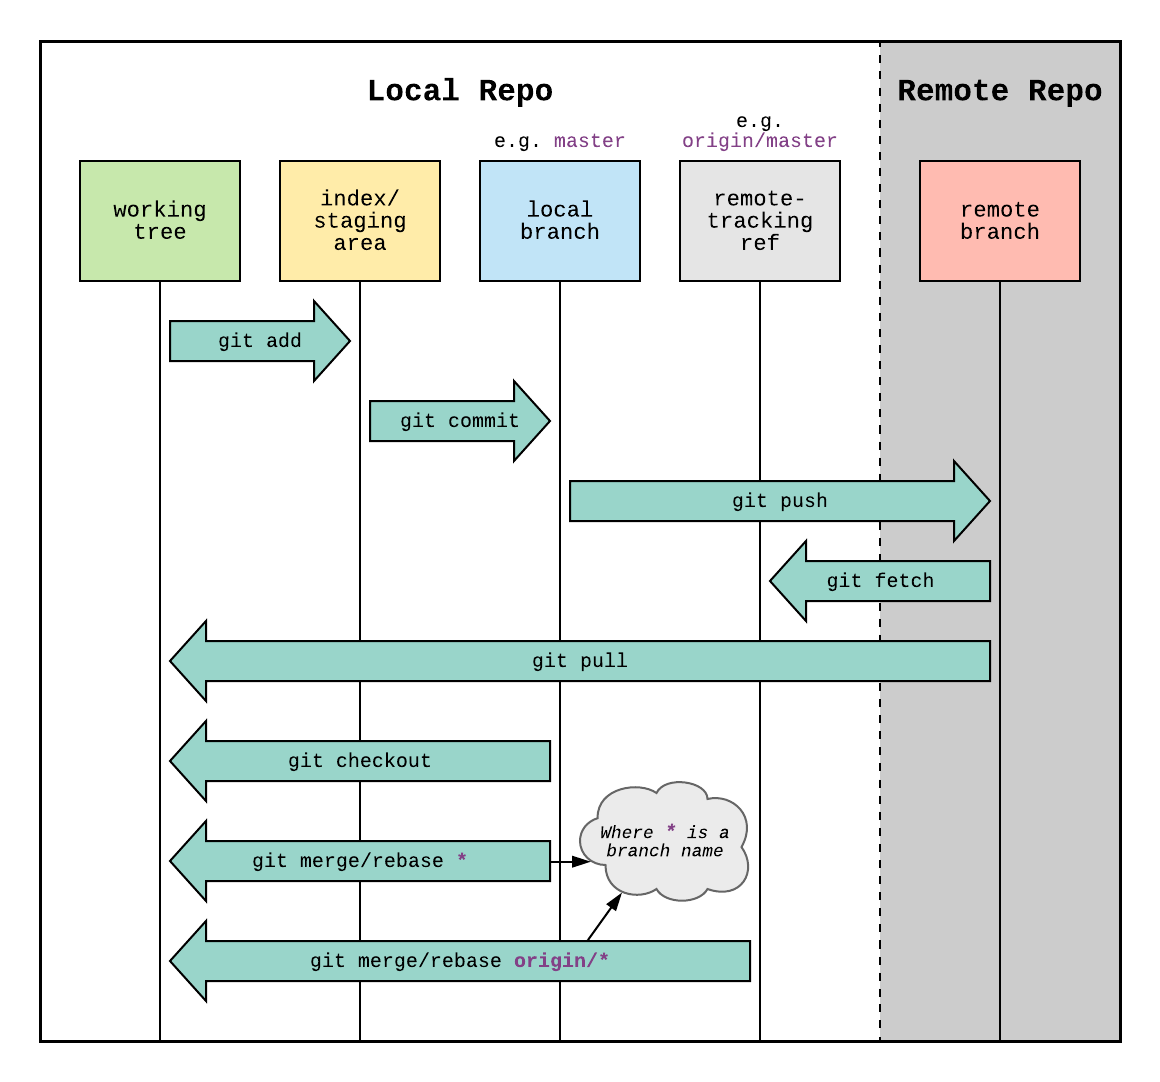
\includegraphics[width=0.6\textwidth]{imgs/github_areas_flow.png}
\caption{Fluxo gráfico de trabalho com repositório remoto.}
\label{fig:github_areas_flow}
\end{figure}
    

    \newpage
\section{Branching e Merging}

O uso de branches (ramificações) é um dos recursos mais poderosos do Git para organizar o desenvolvimento de projetos colaborativos. Branches permitem que diferentes funcionalidades, correções ou experimentos sejam desenvolvidos de forma independente, sem afetar o código principal do projeto. Após o desenvolvimento e testes, as alterações podem ser integradas ao projeto principal por meio do processo de merge (mesclagem).

\subsection{Introdução aos Branches}

Um branch é uma linha de desenvolvimento separada dentro do repositório Git. Por padrão, todo repositório possui um branch principal chamado \texttt{main} (ou \texttt{master}). Ao criar branches, você pode trabalhar em novas funcionalidades, corrigir bugs ou testar ideias sem interferir no código estável do projeto.

Branches são especialmente úteis em equipes, pois cada membro pode trabalhar em sua própria tarefa e, depois de pronta, integrar as alterações ao branch principal.

\subsection{Criando e Mudando de Branch}

Para criar um novo branch, utilize o comando:

\begin{lstlisting}[style=shellstyle]
git branch nome-da-branch
\end{lstlisting}

Para alternar para o branch criado:

\begin{lstlisting}[style=shellstyle]
git checkout nome-da-branch
\end{lstlisting}

Ou, de forma combinada:

\begin{lstlisting}[style=shellstyle]
git checkout -b nome-da-branch
\end{lstlisting}

Exemplo: Para desenvolver uma nova funcionalidade de simulação, crie um branch chamado \texttt{feature/simulacao}:

\begin{lstlisting}[style=shellstyle]
git checkout -b feature/simulacao
\end{lstlisting}

\subsection{Mesclando Branches}

Após finalizar o desenvolvimento em um branch, é necessário integrar as alterações ao branch principal. Isso é feito com o comando \texttt{merge}:

\begin{lstlisting}[style=shellstyle]
git checkout main
git merge feature/simulacao
\end{lstlisting}

O Git irá combinar as alterações do branch \texttt{feature/simulacao} ao branch \texttt{main}. Se não houver conflitos, o merge será realizado automaticamente.

\subsection{Resolvendo Conflitos de Merge}

Conflitos de merge ocorrem quando duas ou mais pessoas modificam a mesma linha de um arquivo em branches diferentes. O Git sinaliza o conflito e pede que o usuário escolha qual versão manter.

Ao realizar um merge e encontrar um conflito, o arquivo afetado exibirá marcações como:

\begin{verbatim}
<<<<<<< HEAD
Conteúdo da branch atual
=======
Conteúdo da branch a ser mesclado
>>>>>>> feature/simulacao
\end{verbatim}

Para resolver o conflito, edite o arquivo, escolha o conteúdo correto e remova as marcações. Depois, finalize o merge:

\begin{lstlisting}[style=shellstyle]
git add arquivo-afetado.ext
git commit -m "Resolve conflito de merge"
\end{lstlisting}

\subsection{Rebasing (Opcional)}

O rebase é uma alternativa ao merge para integrar alterações de um branch ao outro. Ele reorganiza o histórico de commits, tornando-o mais linear. O comando básico é:

\begin{lstlisting}[style=shellstyle]
git checkout feature/simulacao
git rebase main
\end{lstlisting}

O rebase é útil para manter um histórico limpo, mas deve ser usado com cautela em projetos colaborativos, pois pode reescrever o histórico de commits.

\subsection{Exemplo Prático: Fluxo de Trabalho com Branches de Funcionalidade}

Imagine que sua equipe está desenvolvendo um projeto de simulação de voo e precisa adicionar uma nova funcionalidade para calcular a altitude máxima.

\begin{enumerate}
    \item \textbf{Criar um branch para a funcionalidade:}
    \begin{lstlisting}[style=shellstyle]
git checkout -b feature/altitude-maxima
    \end{lstlisting}
    \item \textbf{Desenvolver e commitar as alterações:}
    \begin{lstlisting}[style=shellstyle]
git add simulacao.m
git commit -m "Adiciona cálculo de altitude máxima"
    \end{lstlisting}
    \item \textbf{Mesclar o branch ao principal:}
    \begin{lstlisting}[style=shellstyle]
git checkout main
git merge feature/altitude-maxima
    \end{lstlisting}
    \item \textbf{Resolver conflitos, se houver, e finalizar o merge:}
    \begin{lstlisting}[style=shellstyle]
git add simulacao.m
git commit -m "Resolve conflito e integra cálculo de altitude máxima"
    \end{lstlisting}
\end{enumerate}

Esse fluxo permite que diferentes funcionalidades sejam desenvolvidas em paralelo, testadas e integradas ao projeto principal de forma organizada e segura.




    \newpage
\section{Colaboração e Trabalho em Equipe}

O Git é uma ferramenta poderosa para facilitar o trabalho colaborativo em projetos, permitindo que equipes trabalhem simultaneamente em diferentes partes de um projeto sem conflitos e com total rastreabilidade. Nesta seção, exploraremos como o Git pode ser utilizado para gerenciar contribuições de diferentes membros da equipe, revisar código e adotar boas práticas para garantir a eficiência e a organização do trabalho em grupo.

\subsection{Pull Requests}

O Pull Request (PR) é uma funcionalidade oferecida por plataformas como GitHub e GitLab que permite que um colaborador proponha alterações para um repositório. Ele é amplamente utilizado em projetos colaborativos para integrar contribuições de forma controlada e revisada.

O fluxo básico de um Pull Request é o seguinte:
\begin{enumerate}
    \item O colaborador cria uma nova branch para desenvolver uma funcionalidade ou corrigir um problema.
    \item Após realizar as alterações e fazer os commits, o colaborador envia a branch para o repositório remoto.
    \item No repositório remoto, o colaborador abre um Pull Request, descrevendo as alterações realizadas e o motivo delas.
    \item Outros membros da equipe revisam o Pull Request, sugerem melhorias e aprovam as alterações.
    \item Após a aprovação, as alterações são integradas à branch principal (\texttt{main} ou \texttt{master}) por meio de um merge.
\end{enumerate}

Os Pull Requests são uma excelente forma de garantir que todas as alterações sejam revisadas antes de serem integradas ao projeto, promovendo a qualidade do código e a colaboração entre os membros da equipe.

\subsection{Revisão de Código}

A revisão de código é uma etapa essencial no trabalho colaborativo, pois permite que os membros da equipe avaliem as contribuições uns dos outros, identifiquem erros, sugiram melhorias e garantam a consistência do projeto. Durante a revisão de um Pull Request, os revisores devem:
\begin{itemize}
    \item Verificar se o código segue os padrões e boas práticas estabelecidos pela equipe.
    \item Garantir que as alterações não introduzam erros ou quebras no projeto.
    \item Testar as novas funcionalidades ou correções, quando aplicável.
    \item Sugerir melhorias para tornar o código mais eficiente, legível ou organizado.
\end{itemize}

A revisão de código não deve ser vista como uma crítica pessoal, mas como uma oportunidade de aprendizado e melhoria contínua para toda a equipe. Ferramentas como comentários em Pull Requests no GitHub ou GitLab tornam esse processo mais eficiente e colaborativo.

\subsection{Boas Práticas em Projetos de Equipe}

Para garantir o sucesso de um projeto colaborativo, é importante adotar boas práticas no uso do Git. Algumas recomendações incluem:
\begin{itemize}
    \item \textbf{Criar branches para cada tarefa:} Cada funcionalidade ou correção deve ser desenvolvida em uma branch separada, com um nome descritivo, como \texttt{feature/simulacao} ou \texttt{bugfix/corrigir-grafico}.
    \item \textbf{Escrever mensagens de commit claras:} Cada commit deve ter uma mensagem que explique de forma objetiva o que foi alterado, como \texttt{"Adiciona função para calcular resistência do ar"}.
    \item \textbf{Sincronizar frequentemente:} Antes de iniciar uma nova tarefa, atualize sua branch local com as alterações mais recentes da branch principal para evitar conflitos.
    \item \textbf{Resolver conflitos de forma colaborativa:} Quando conflitos de versão ocorrerem, discuta com os membros da equipe para decidir a melhor forma de resolvê-los.
    \item \textbf{Revisar e testar antes de integrar:} Antes de fazer o merge de uma branch, certifique-se de que todas as alterações foram revisadas e testadas.
\end{itemize}

Essas práticas ajudam a manter o projeto organizado, reduzir erros e promover um ambiente de trabalho colaborativo e produtivo.

\subsection{Exemplo Prático: Contribuindo para um Repositório Compartilhado}

%% ber - NECESSITA SER TOTALMENTE REFEITO E PENSADO, isso é um exemplo do gpt

Vamos considerar um exemplo prático de colaboração em um projeto de simulação de voo atmosférico. Suponha que você e sua equipe estão desenvolvendo um modelo no MATLAB/Simulink e precisam adicionar uma nova funcionalidade para calcular a resistência do ar.

\subsubsection*{Passo 1: Criar uma branch para a tarefa}

No terminal, crie uma nova branch para desenvolver a funcionalidade:
\begin{lstlisting}[style=shellstyle]
git checkout -b feature/resistencia-ar
\end{lstlisting}

\subsubsection*{Passo 2: Fazer as alterações e commits}

Implemente a funcionalidade no código e registre as alterações com commits claros:
\begin{lstlisting}[style=shellstyle]
git add simulacao.m
git commit -m "Adiciona função para calcular resistência do ar"
\end{lstlisting}

\subsubsection*{Passo 3: Enviar a branch para o repositório remoto}

Envie a branch para o repositório remoto para compartilhar seu trabalho:
\begin{lstlisting}[style=shellstyle]
git push origin feature/resistencia-ar
\end{lstlisting}

\subsubsection*{Passo 4: Abrir um Pull Request}

No GitHub ou GitLab, abra um Pull Request para a branch \texttt{feature/resistencia-ar}, descrevendo as alterações realizadas.

\subsubsection*{Passo 5: Revisar e integrar as alterações}

Os membros da equipe revisam o Pull Request, sugerem melhorias e, após a aprovação, fazem o merge da branch na branch principal:
\begin{lstlisting}[style=shellstyle]
git checkout main
git merge feature/resistencia-ar
\end{lstlisting}

\subsubsection*{Passo 6: Atualizar o repositório local}

Após o merge, atualize seu repositório local para refletir as alterações mais recentes:
\begin{lstlisting}[style=shellstyle]
git pull origin main
\end{lstlisting}

Com esse fluxo, a equipe pode colaborar de forma eficiente, garantindo que todas as contribuições sejam revisadas, testadas e integradas de maneira

    \newpage

\section{Recuperação de Versões e Versionamento}

\subsection{Visualização do Histórico de Commits}

O histórico de commits permite acompanhar todas as alterações feitas no projeto, quem realizou cada mudança e quando. Para visualizar o histórico completo, utilize:

\begin{lstlisting}[style=shellstyle]
git log
\end{lstlisting}

O comando \texttt{git log} exibe uma lista cronológica de commits, apresentando informações como hash único, autor, data e mensagem de cada alteração. Ao executar este comando, você observará que o commit mais recente está identificado pela referência HEAD. O HEAD é um ponteiro que indica a posição atual no histórico do repositório, apontando para o commit em que você está trabalhando no momento, geralmente correspondendo ao último commit do branch atual.

No GitHub, acesse a aba Commits do repositório para ver o histórico online, incluindo autor, data e mensagem de cada commit.

\subsection{Recuperação de Arquivos ou Versões Anteriores}

Se for necessário restaurar um arquivo (caso ele tenha sido deletado, por exemplo), utilize:

\begin{lstlisting}[style=shellstyle]
git checkout <hash-do-commit> -- <nome-do-arquivo>
\end{lstlisting}

Caso seja necessário restaurar todo o projeto para um estado anterior, utilize:

\begin{lstlisting}[style=shellstyle]
git checkout <hash-do-commit>
\end{lstlisting}

Nesse caso, tenha atenção: ao fazer isso, o Git colocará o repositório em um estado chamado \textbf{detached HEAD}. Isso significa que você estará apenas visitando um commit antigo, e não estará mais no seu branch atual (por exemplo, \texttt{main} ou \texttt{develop}).  

Se o seu objetivo for apenas consultar o estado do projeto ou recuperar arquivos antigos, isso não é um problema. No entanto, se você fizer alterações e criar novos commits nesse estado, eles não estarão vinculados a nenhum branch e poderão ser perdidos ao trocar de branch.  

Se você quiser apenas olhar um commit antigo, depois de terminar, basta voltar para o seu branch principal com:

\begin{lstlisting}[style=shellstyle]
git checkout main
\end{lstlisting}

Por outro lado, se o objetivo for continuar trabalhando a partir de um commit antigo, o recomendado é criar um novo branch antes de fazer alterações. Isso garante que seus novos commits fiquem salvos com segurança:

\begin{lstlisting}[style=shellstyle]
git checkout -b meu-novo-branch <hash-do-commit>
\end{lstlisting}

Dessa forma, você cria um branch começando do commit escolhido e evita problemas com o modo detached HEAD.  

\subsection{Reversão de Commits (Undo/Revert/Reset)}

Para desfazer alterações no histórico do Git, existem diferentes comandos dependendo do contexto e da severidade necessária.

Para reverter um commit que já foi enviado ao repositório remoto, utilize o comando git revert. Este comando cria um novo commit que desfaz as alterações do commit especificado, sendo seguro para uso em commits públicos:

\begin{lstlisting}[style=shellstyle]
git revert <hash-do-commit>
\end{lstlisting}

Para commits que ainda não foram enviados ao repositório remoto, pode-se utilizar o comando \texttt{git reset}. Este comando possui três modos principais de operação, que diferem no tratamento das alterações não commitadas:

\begin{lstlisting}[style=shellstyle]
git reset --soft <hash-do-commit>
\end{lstlisting}

O modo \texttt{--soft} move o ponteiro HEAD para o commit especificado, mas mantém todas as alterações subsequentes na área de staging, permitindo que você refaça o commit com mudanças.

\begin{lstlisting}[style=shellstyle]
git reset --mixed <hash-do-commit>
\end{lstlisting}

O modo \texttt{--mixed} (padrão quando nenhuma opção é especificada) move o HEAD e desfaz o staging das alterações, mas mantém as modificações no diretório de trabalho.

\begin{lstlisting}[style=shellstyle]
git reset --hard <hash-do-commit>
\end{lstlisting}

O modo \texttt{--hard} move o HEAD e descarta todas as alterações não commitadas, retornando o diretório de trabalho exatamente ao estado do commit especificado. Este comando deve ser usado com cautela, pois pode eliminar permanentemente trabalho não salvo.

No GitHub, a reversão também pode ser realizada através da interface web, que automaticamente cria um novo commit revertendo as alterações indesejadas.

\subsection{Comparação entre Versões (Diff)}

Para comparar as diferenças entre dois commits, utilize:

\begin{lstlisting}[style=shellstyle]
git diff <hash1> <hash2>
\end{lstlisting}

No GitHub, selecione dois commits ou branches e use a aba Compare para visualizar as diferenças entre eles.

\subsection{Criação de Tags e Releases}

Tags marcam pontos importantes no histórico, como versões estáveis. Para criar uma tag:

\begin{lstlisting}[style=shellstyle]
git tag -a v1.0 -m "Versão 1.0"
git push origin v1.0
\end{lstlisting}

No GitHub, utilize a aba Releases para criar e gerenciar versões do projeto.

\subsection{Uso de Branches para Versionamento Seguro}

Branches permitem desenvolver novas funcionalidades ou corrigir erros sem afetar o código principal. Para criar um branch:

\begin{lstlisting}[style=shellstyle]
git checkout -b nome-do-branch
\end{lstlisting}

No GitHub, branches são facilmente visualizados e gerenciados na interface do repositório.

\subsection{Auditoria e Rastreabilidade (Blame, Log Detalhado)}

Para identificar quem modificou cada linha de um arquivo, utilize:

\begin{lstlisting}[style=shellstyle]
git blame <nome-do-arquivo>
\end{lstlisting}

O comando \texttt{git log} também pode ser usado com filtros para auditoria detalhada:

\begin{lstlisting}[style=shellstyle]
git log -p <nome-do-arquivo>
\end{lstlisting}

No GitHub, use a opção Blame na visualização de arquivos para

    \newpage
\section{Boas Práticas}

Adotar boas práticas no uso do Git é essencial para garantir a organização, a rastreabilidade e a eficiência dos projetos colaborativos. Nesta seção, abordamos recomendações para escrever mensagens de commit claras, organizar repositórios, evitar erros comuns e implementar metodologias de desenvolvimento como o GitFlow.

\subsection{Escrevendo Bons Commit Messages}

Mensagens de commit bem escritas facilitam o entendimento do histórico do projeto e ajudam toda a equipe a acompanhar as alterações. Recomendações:
\begin{itemize}
    \item Seja objetivo e claro: descreva o que foi alterado e por quê.
    \item Evite mensagens genéricas como \texttt{"Update"} ou \texttt{"Correções"}.
    \item Se necessário, adicione uma descrição mais detalhada após a primeira linha.
\end{itemize}

\subsection{Organizando Repositórios}

Um repositório bem organizado facilita a navegação e o entendimento do projeto. Dicas:
\begin{itemize}
    \item Mantenha uma estrutura de pastas lógica (ex: \texttt{src/}, \texttt{docs/}, \texttt{data/}).
    \item Utilize arquivos \texttt{README.md} para documentar o objetivo do projeto e instruções de uso.
    \item Adote o \texttt{.gitignore} para evitar versionar arquivos desnecessários ou temporários.
    \item Padronize nomes de arquivos e pastas.
\end{itemize}

\subsection{Erros Comuns a Evitar}

Alguns erros podem comprometer a organização e a colaboração no projeto:
\begin{itemize}
    \item Versionar arquivos grandes ou gerados automaticamente (ex: \texttt{.mat}, \texttt{.exe}, \texttt{.log}).
    \item Realizar commits diretamente na branch principal sem revisão.
    \item Não atualizar o repositório local antes de iniciar novas tarefas.
    \item Mensagens de commit vagas ou sem contexto.
    \item Não resolver conflitos de merge corretamente.
\end{itemize}

% \subsection{Assinatura de Commits (Opcional)}

% Assinar commits com uma chave GPG garante autenticidade e segurança, especialmente em projetos públicos ou críticos. Para configurar:
% \begin{lstlisting}[style=shellstyle]
% git config --global user.signingkey <ID-da-chave>
% git commit -S -m "Mensagem assinada"
% \end{lstlisting}
% Mais detalhes podem ser encontrados na documentação oficial do Git: \url{https://git-scm.com/book/en/v2/Git-Tools-Signing-Your-Work}

\subsection{GitFlow - Metodologia de Desenvolvimento Colaborativo}

O \textbf{GitFlow} é uma metodologia que define um fluxo de trabalho estruturado para equipes que usam Git. Ele organiza o desenvolvimento em diferentes tipos de branches, cada um com uma finalidade específica:
\begin{itemize}
    \item \texttt{main} (ou \texttt{master}): branch principal, sempre estável.
    \item \texttt{develop}: branch de desenvolvimento, onde novas funcionalidades são integradas antes de serem lançadas.
    \item \texttt{feature/*}: branches para desenvolvimento de novas funcionalidades.
    \item \texttt{release/*}: branches para preparação de novas versões.
    \item \texttt{hotfix/*}: branches para correção rápida de bugs em produção.
\end{itemize}

O GitFlow facilita o gerenciamento de múltiplas tarefas simultâneas, garante que o código principal permaneça estável e organiza o processo de lançamento de versões.

Para implementar o GitFlow, existem extensões e ferramentas que automatizam o processo. O documento original do GitFlow pode ser acessado em: \url{https://nvie.com/posts/a-successful-git-branching-model/}

Adotar o GitFlow em projetos colaborativos aumenta a produtividade, reduz conflitos e torna o ciclo de desenvolvimento mais previsível.

\begin{quote}
\textbf{Nota:}
A leitura do documento oficial do GitFlow é fortemente recomendada. Uma boa compreensão dessa metodologia colaborativa esclarece o funcionamento de um repositório Git bem estruturado e contribui para o sucesso de projetos versionados em equipe.
\end{quote}



    \newpage
\section{Exercícios Práticos}

Esta seção apresenta exercícios para consolidar os conceitos abordados ao longo da apostila. Os exercícios estão divididos em níveis de dificuldade e incluem um mini-projeto colaborativo, permitindo que você pratique desde os comandos básicos até situações reais de trabalho em equipe com Git.

Para todos os exercícios dessa seção, o ambiente integrado de desenvolvimento Visual Studio Code será utilizado.

\subsection{Nível Iniciante}

\subsubsection{Criar um Repositório Local}
\begin{itemize}
    \item Crie uma pasta chamada \texttt{meu\_projeto\_git} em seu computador.

    \begin{figure}[H]
        \centering
        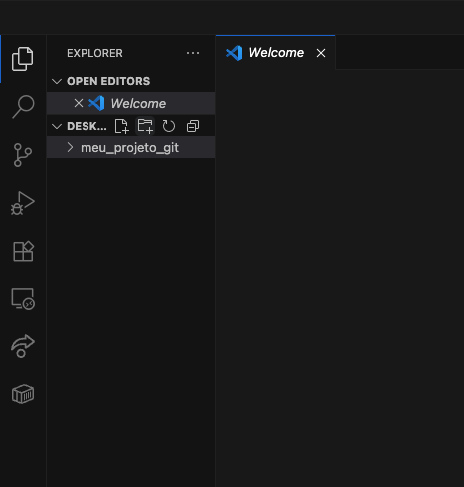
\includegraphics[width=0.6\textwidth]{imgs/tutorial_github/ex01_01.png}
        \label{fig:ex01_01}
        \caption{Solução do exercício 01: Criando a pasta meu\_projeto\_git no VS Code.}
    \end{figure}

    \begin{figure}[H]
        \centering
        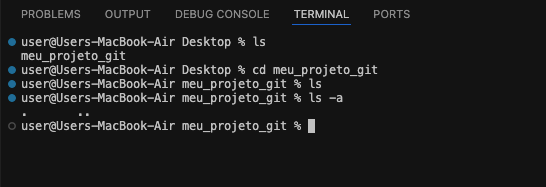
\includegraphics[width=0.6\textwidth]{imgs/tutorial_github/ex01_01_1.png}
        \label{fig:ex01_01_01}
        \caption{Solução do exercício 01: Utilizando o terminal do VS Code e alguns comandos para entrar na pasta meu\_projeto\_git e verificar os arquivos da pasta.}
    \end{figure}


    \item Inicialize um repositório Git na pasta:
    \begin{lstlisting}[style=shellstyle]
git init
    \end{lstlisting}


    \begin{figure}[H]
        \centering
        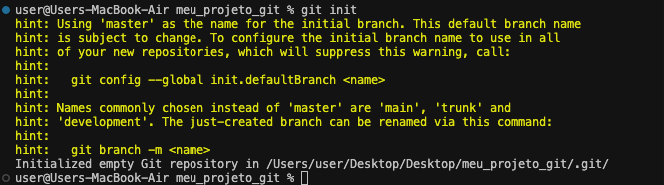
\includegraphics[width=0.6\textwidth]{imgs/tutorial_github/ex01_02.png}
        \label{fig:ex01_02}
        \caption{Solução do exercício 01: Inicializando o repositório git.}
    \end{figure}
    
    \item Verifique o status do repositório:
    \begin{lstlisting}[style=shellstyle]
git status
    \end{lstlisting}

    \begin{figure}[H]
        \centering
        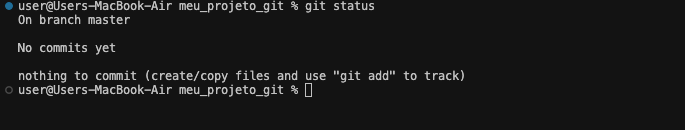
\includegraphics[width=0.6\textwidth]{imgs/tutorial_github/ex01_03.png}
        \label{fig:ex01_03}
        \caption{Solução do exercício 01: Verificando o status do repositório.}
    \end{figure}
    
\end{itemize}



\subsubsection{Rastrear Arquivos e Fazer Commits}
\begin{itemize}
    \item Crie um arquivo chamado \texttt{README.md} e escreva uma breve descrição do projeto.

       \begin{figure}[H]
        \centering
        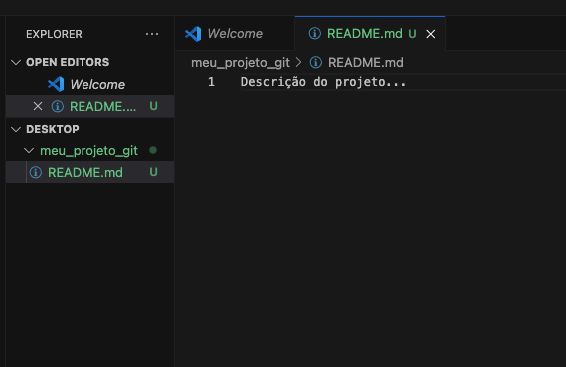
\includegraphics[width=0.6\textwidth]{imgs/tutorial_github/ex02_01.png}
        \label{fig:ex02_01}
        \caption{Solução do exercício 02: Criando o arquivo README.md.}
    \end{figure}

    \begin{figure}[H]
        \centering
        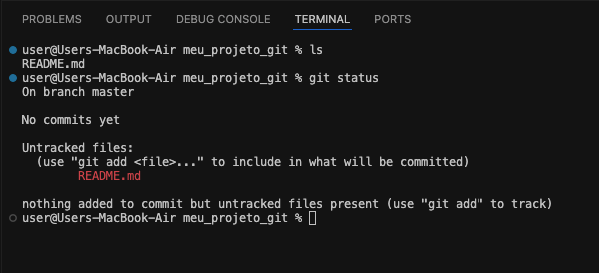
\includegraphics[width=0.6\textwidth]{imgs/tutorial_github/ex02_01_01.png}
        \label{fig:ex02_01_01}
        \caption{Solução do exercício 02: Git status retorna que README.md é um novo arquivo que precisa ser adicionado ao repositório git.}
    \end{figure}
    
    \item Adicione o arquivo ao staging area:
    \begin{lstlisting}[style=shellstyle]
git add README.md
    \end{lstlisting}
    \item Faça um commit com uma mensagem clara:
    \begin{lstlisting}[style=shellstyle]
git commit -m "Adiciona README inicial"
    \end{lstlisting}

    \begin{figure}[H]
        \centering
        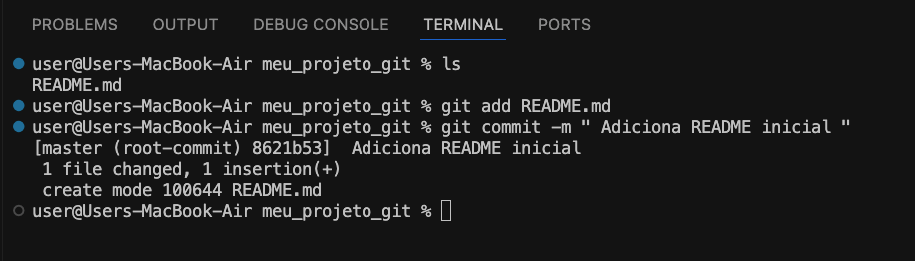
\includegraphics[width=0.6\textwidth]{imgs/tutorial_github/ex02_02.png}
        \label{fig:ex02_02}
        \caption{Solução do exercício 02: Adicionando README.md e fazendo o commit.}
    \end{figure}
    
    \item Crie mais um arquivo (ex: \texttt{codigo.m}) e repita o processo:
    \begin{lstlisting}[style=shellstyle]
git add codigo.m
git commit -m "Adiciona código MATLAB inicial"
    \end{lstlisting}

    \begin{figure}[H]
        \centering
        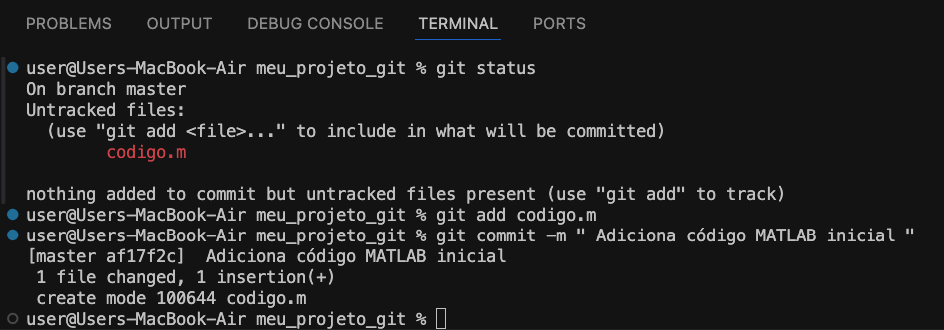
\includegraphics[width=0.6\textwidth]{imgs/tutorial_github/ex02_03.png}
        \label{fig:ex02_03}
        \caption{Solução do exercício 02: Adicionando codigo.m e fazendo o commit.}
    \end{figure}
    
\end{itemize}

\subsubsection{Enviar para um Repositório Remoto}
\begin{itemize}
    \item Crie um repositório remoto no GitHub ou GitLab.

    \begin{figure}[H]
        \centering
        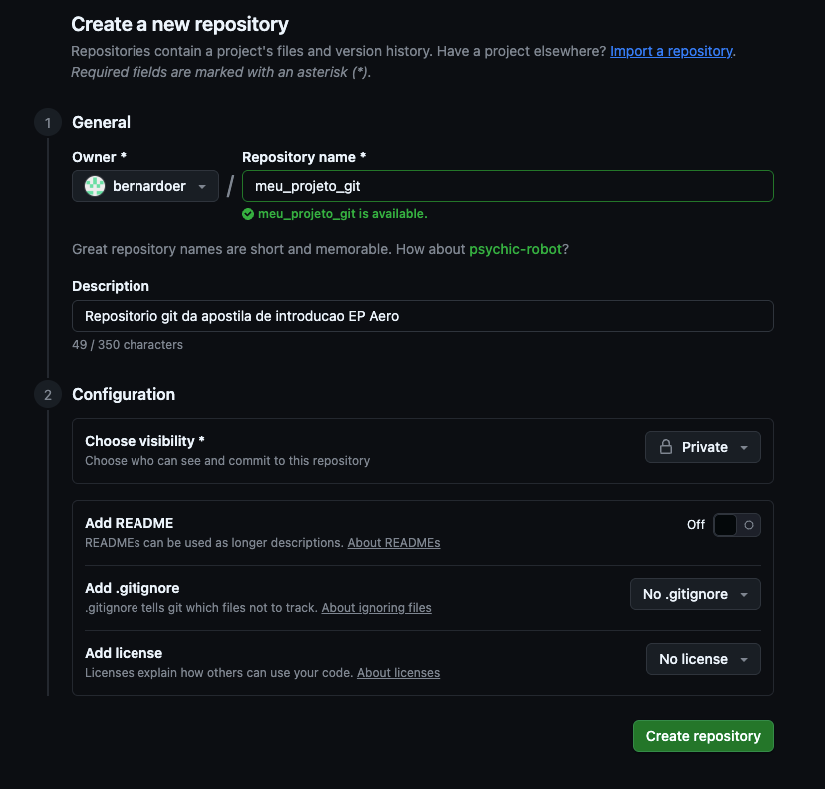
\includegraphics[width=0.6\textwidth]{imgs/tutorial_github/ex03_01.png}
        \label{fig:ex03_01}
        \caption{Solução do exercício 03: Criando o repositório no GitHub.}
    \end{figure}
    
    \item Conecte o repositório local ao remoto:
    \begin{lstlisting}[style=shellstyle]
git remote add origin <URL-do-repositório>
    \end{lstlisting}

    
    \item Envie seus commits para o remoto:
    \begin{lstlisting}[style=shellstyle]
git push origin main
    \end{lstlisting}

    \begin{figure}[H]
        \centering
        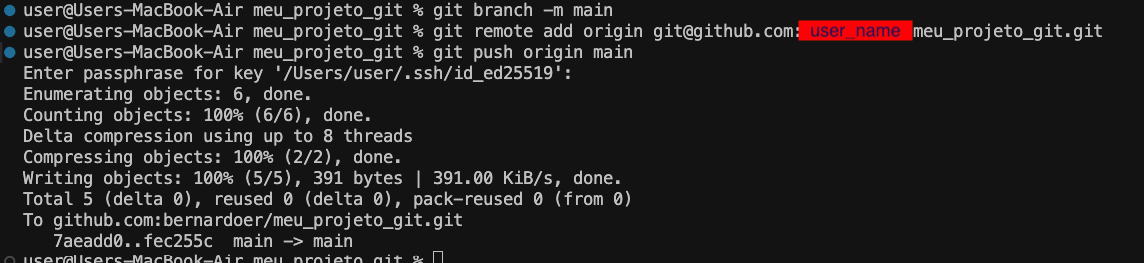
\includegraphics[width=0.6\textwidth]{imgs/tutorial_github/ex03_03.png}
        \label{fig:ex03_02}
        \caption{Solução do exercício 03: Adicionando a branch master no repositório GitHub.}
    \end{figure}
\end{itemize}

\subsection{Nível Intermediário}

\subsubsection{Criar e Mesclar Branches}
\begin{itemize}
    \item Crie um branch chamado \texttt{feature/descricao}:
    \begin{lstlisting}[style=shellstyle]
git checkout -b feature/descricao
    \end{lstlisting}
    \item No novo branch, edite o \texttt{README.md} adicionando mais detalhes sobre o projeto.
    \item Adicione e faça commit das alterações:
    \begin{lstlisting}[style=shellstyle]
git add README.md
git commit -m "Adiciona detalhes ao README"
    \end{lstlisting}
    \item Retorne ao branch principal:
    \begin{lstlisting}[style=shellstyle]
git checkout main
    \end{lstlisting}
    \item Mescle o branch de funcionalidade:
    \begin{lstlisting}[style=shellstyle]
git merge feature/descricao
    \end{lstlisting}
\end{itemize}

 \begin{figure}[H]
        \centering
        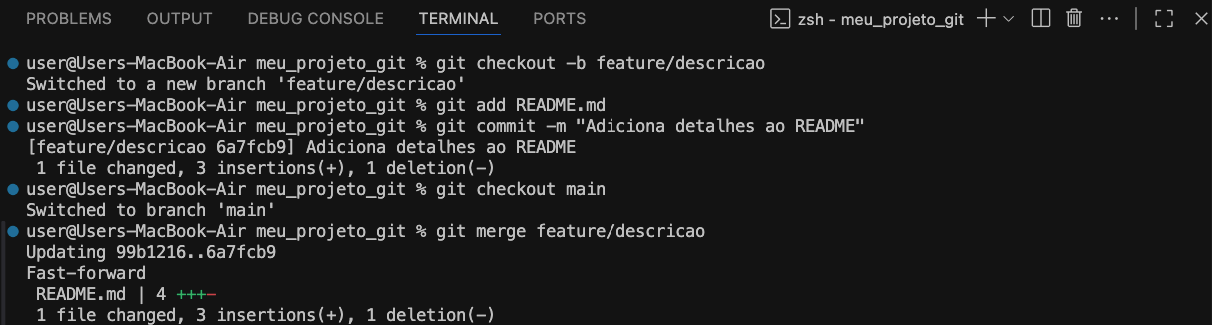
\includegraphics[width=0.6\textwidth]{imgs/tutorial_github/ex04_01.png}
        \label{fig:ex04_01}
        \caption{Solução do exercício 04: Criando feature branch para editar o projeto.}
    \end{figure}

\subsubsection{Resolver Conflitos de Merge}
\begin{itemize}
    \item Simule um conflito editando a mesma linha do \texttt{README.md} em dois branches diferentes.
    \item Tente fazer o merge e, ao encontrar um conflito, edite o arquivo manualmente para resolver.
    \item Após resolver, adicione e faça commit:
    \begin{lstlisting}[style=shellstyle]
git add README.md
git commit -m "Resolve conflito de merge no README"
    \end{lstlisting}
\end{itemize}

\subsubsection{Utilizar Efetivamente o .gitignore}
\begin{itemize}
    \item Crie arquivos temporários (\texttt{.log}, \texttt{.tmp}) na pasta do projeto.
    \item Crie um arquivo \texttt{.gitignore} e adicione regras para ignorar esses arquivos.
    \item Verifique que os arquivos ignorados não aparecem no status:
    \begin{lstlisting}[style=shellstyle]
git status
    \end{lstlisting}
\end{itemize}

\subsection{Mini-Projeto Prático: Gerenciando um Pequeno Projeto de Equipe}

Monte uma equipe de 2 a 4 pessoas e siga os passos abaixo:

\begin{enumerate}
    \item Crie um repositório remoto compartilhado no GitHub ou GitLab.
    \item Cada integrante deve clonar o repositório:
    \begin{lstlisting}[style=shellstyle]
git clone <URL-do-repositório>
    \end{lstlisting}
    \item Divida as tarefas: cada pessoa deve criar um branch para desenvolver uma funcionalidade:
    \begin{lstlisting}[style=shellstyle]
git checkout -b feature/modelo
    \end{lstlisting}
    \item Realize commits frequentes e mensagens claras:
    \begin{lstlisting}[style=shellstyle]
git add <arquivo>
git commit -m "Mensagem clara sobre a alteração"
    \end{lstlisting}
    \item Abra Pull Requests na plataforma para integrar as funcionalidades ao branch principal.
    \item Realize revisões de código e resolva possíveis conflitos de merge.
    \item Ao final, garanta que o projeto esteja organizado, com README atualizado e arquivos desnecessários ignorados pelo \texttt{.gitignore}.
\end{enumerate}

Esses exercícios proporcionam experiência prática com os principais comandos e fluxos de trabalho do Git, preparando você para atuar em projetos reais de engenharia

\subsection{Contribuindo com as apostilas da EP Aero no Github}

Todas as apostilas da EP Aero são disponibilizadas publicamente e de forma gratuita no Github. Os autores da apostila incentivam a contribuição dos leitores para aprimorar o conteúdo, corrigir erros e sugerir melhorias.

Para fazer isso, siga o passo-a-passo a seguir:

\begin{itemize}
        \item Acesse o repositório da apostila no Github: \url{https://github.com/ep-aero-ufsm/apostila-github}
        \item Faça um fork do repositório para sua conta. Para fazer isso, você pode usar a interface web do Github, como mostrado nas figuras \ref{fig:1_fork} e \ref{fig:2_fork}.
\begin{figure}[H]
        \centering
        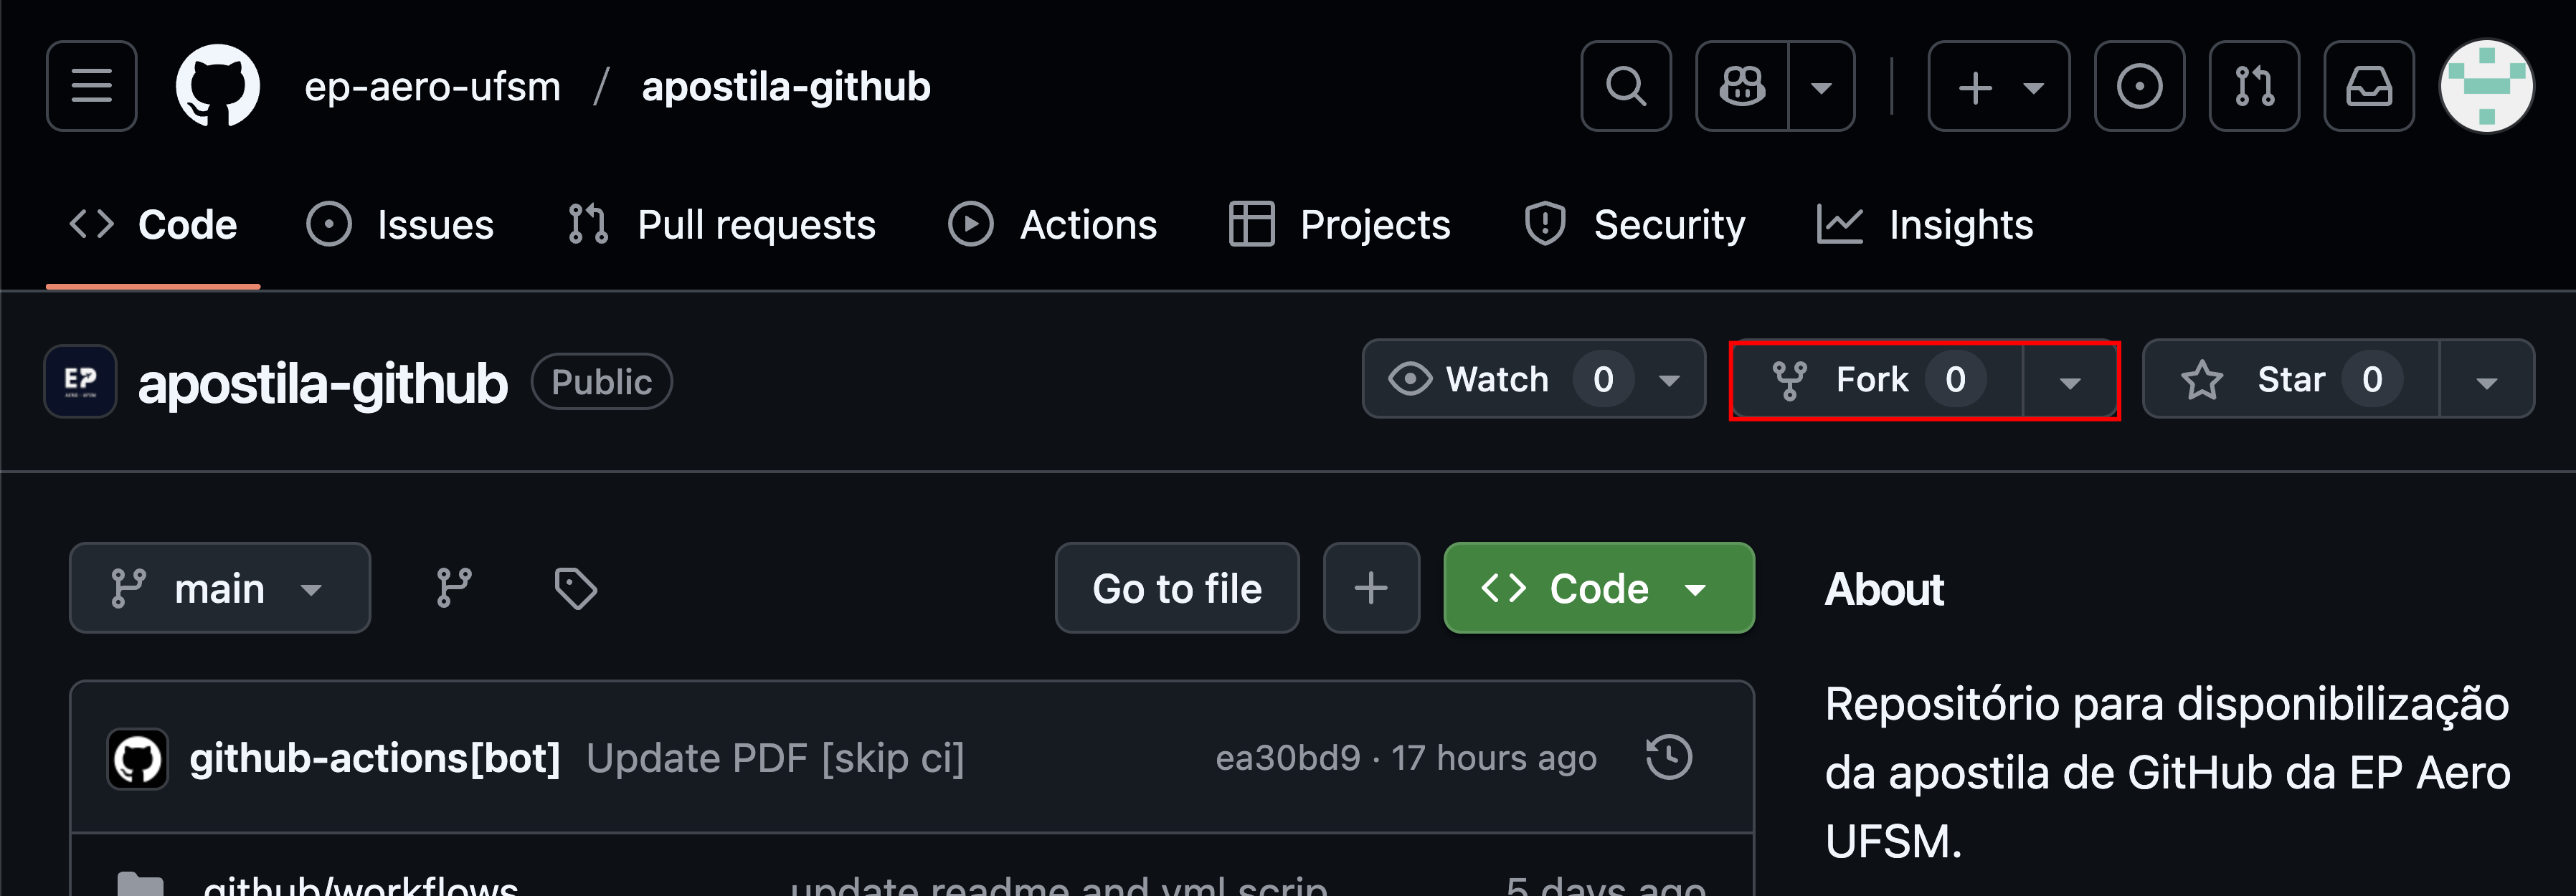
\includegraphics[width=0.6\textwidth]{imgs/tutorial_contribuicao/1_fork.png}
        \caption{Como criar um fork do repositório - etapa 1.}
        \label{fig:1_fork}
    \end{figure}

    \begin{figure}[H]
        \centering
        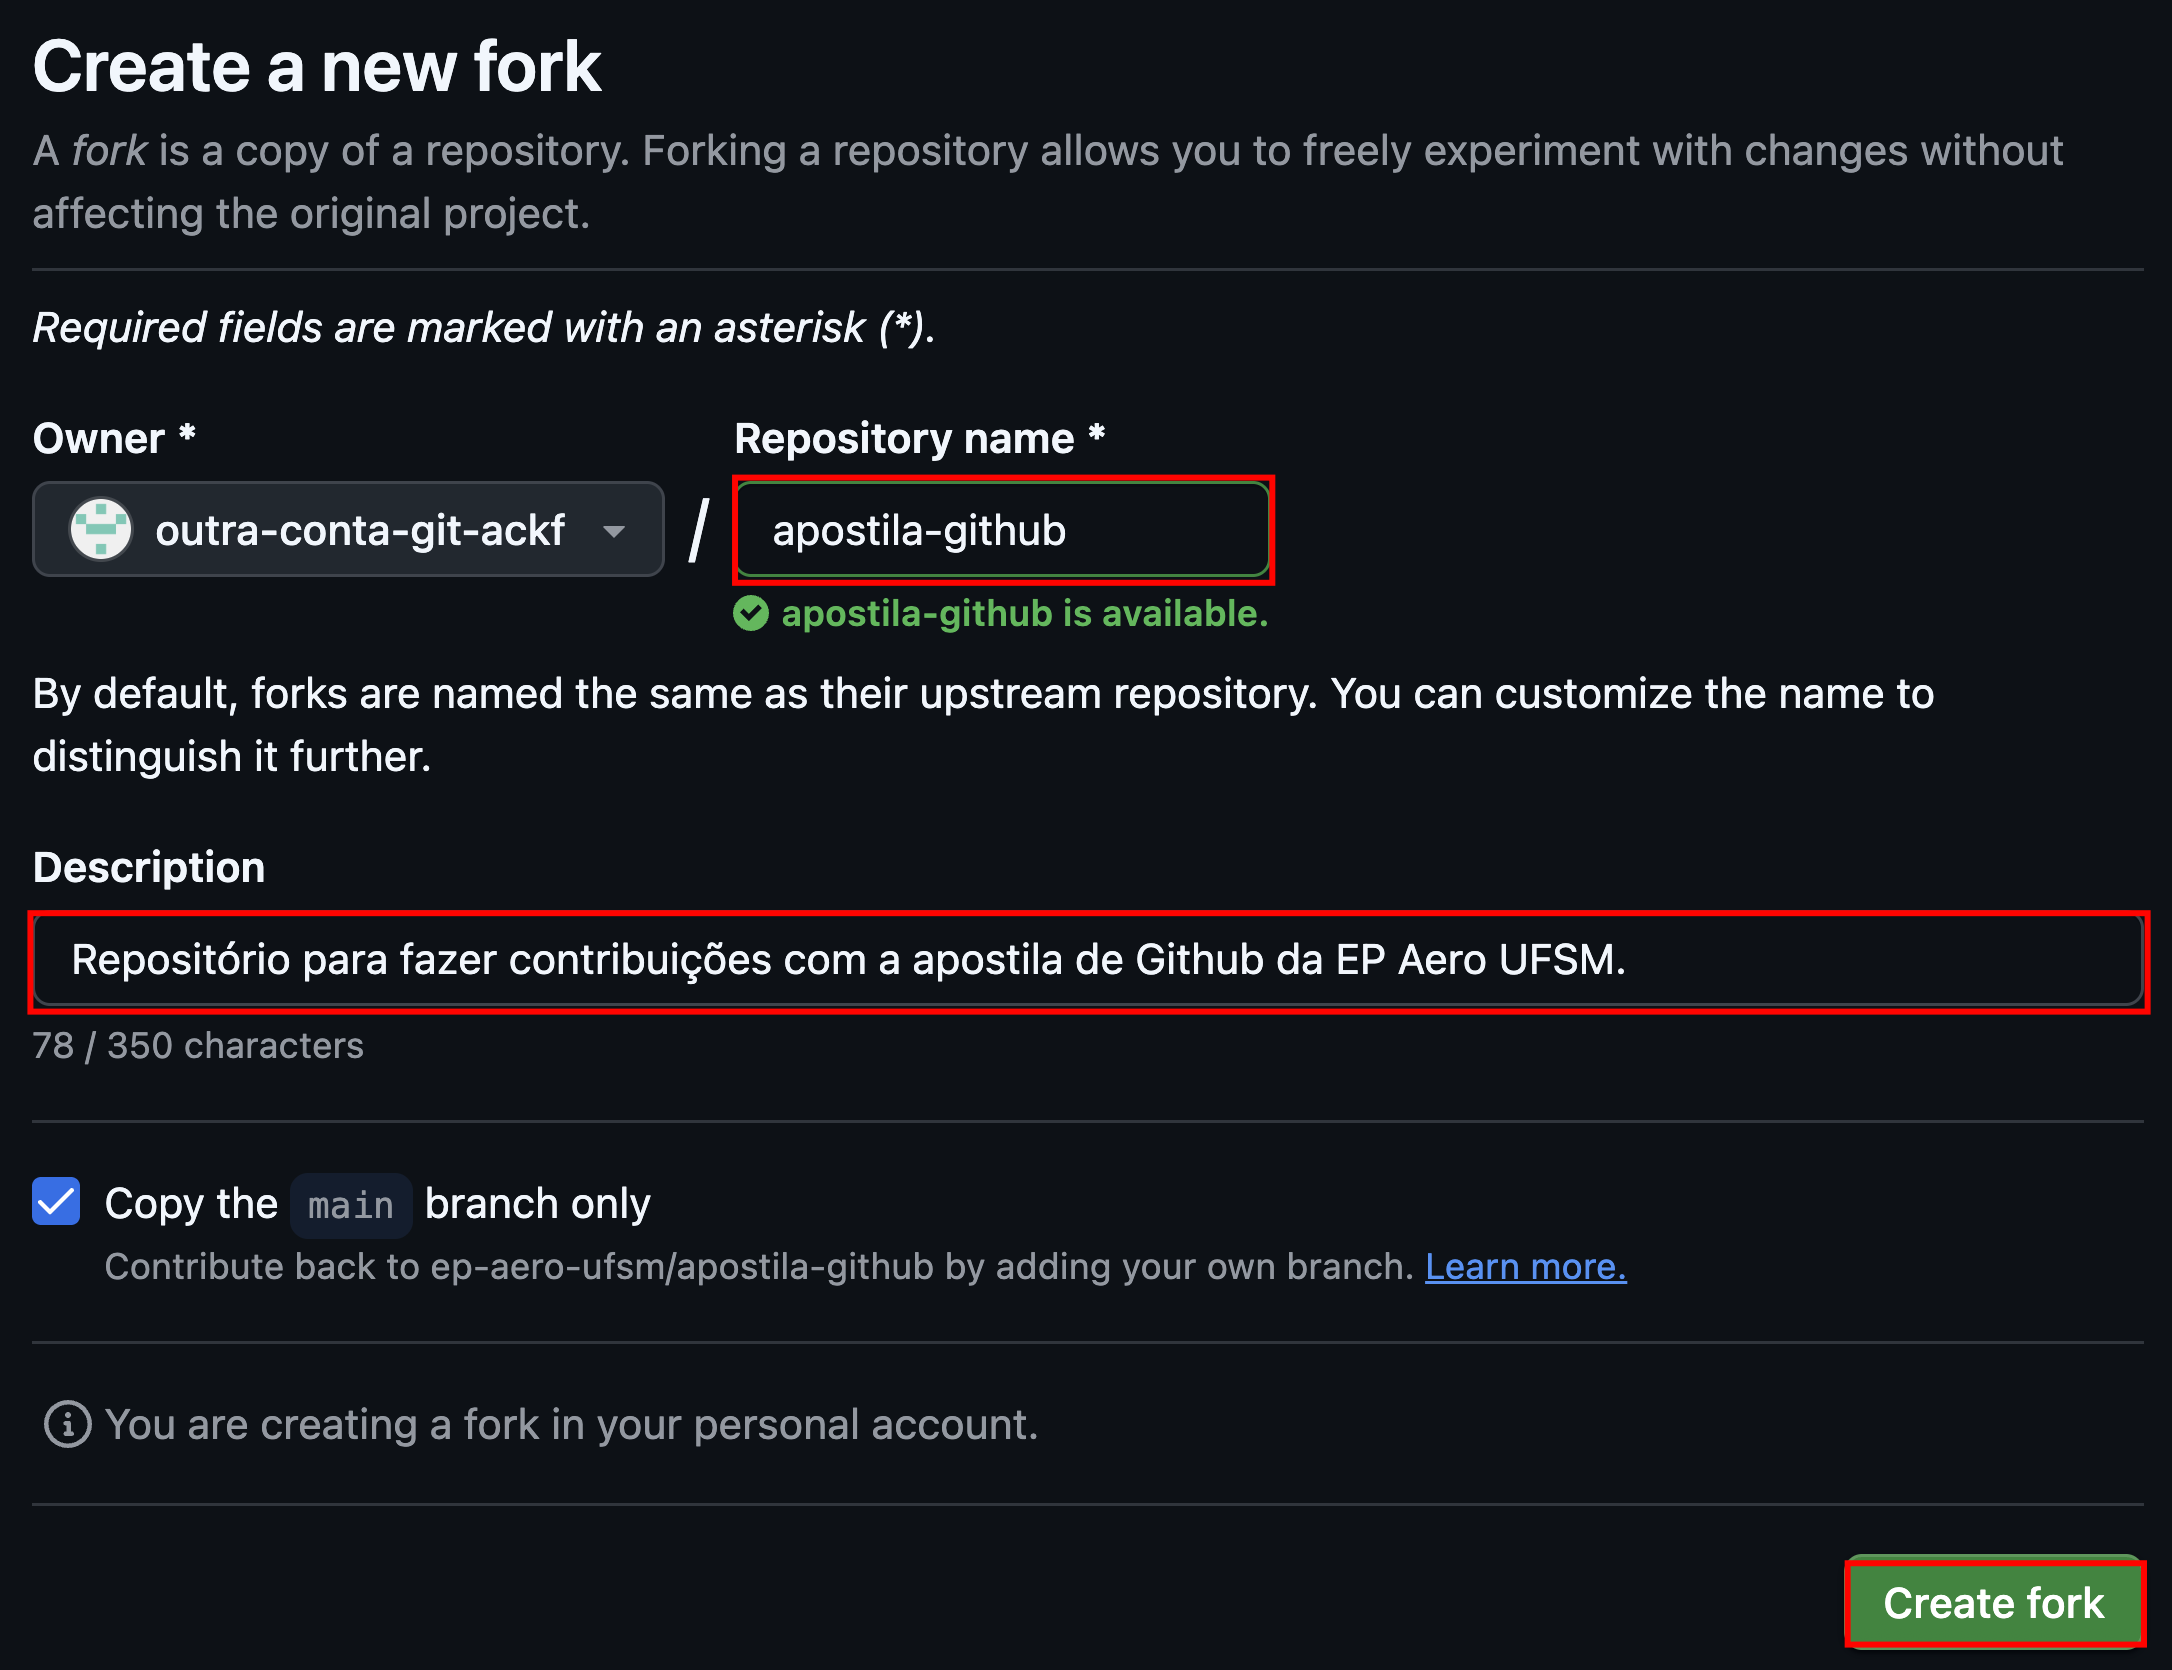
\includegraphics[width=0.6\textwidth]{imgs/tutorial_contribuicao/2_fork.png}
        \caption{Como criar um fork do repositório - etapa 2.}
        \label{fig:2_fork}
    \end{figure}

        \item Você pode alterar o nome do repositório e a descrição como desejar. Neste exemplo, o nome do repositório foi mantido igual (apostila-github).
        \item Clone o repositório forkado para seu computador. Nesse momento, você pode usar o link SSH caso já tenha configurado:
        \begin{lstlisting}[style=shellstyle]
git clone git@github.com:seu-usuario/apostila-github.git
        \end{lstlisting}
        \item Crie um branch para sua contribuição:
        \begin{lstlisting}[style=shellstyle]
git checkout -b minha-contribuicao
        \end{lstlisting}
        \item Faça as alterações desejadas (correções, melhorias, adição de conteúdo). Por exemplo, foi identificado que a exibição dos nomes dos autores estava incorreta no README do repositório, como mostrado na figura \ref{fig:README_antes_modif}.

        \begin{figure}[H]
        \centering
        
\includegraphics[width=0.6\textwidth]{imgs/tutorial_contribuicao/README_antes_modif.png}
        \caption{README com erro de formatação.}
        \label{fig:README_antes_modif}
    \end{figure}

        \item Na sequência, foram feitas as seguintes modificações:

        \begin{figure}[H]
        \centering
        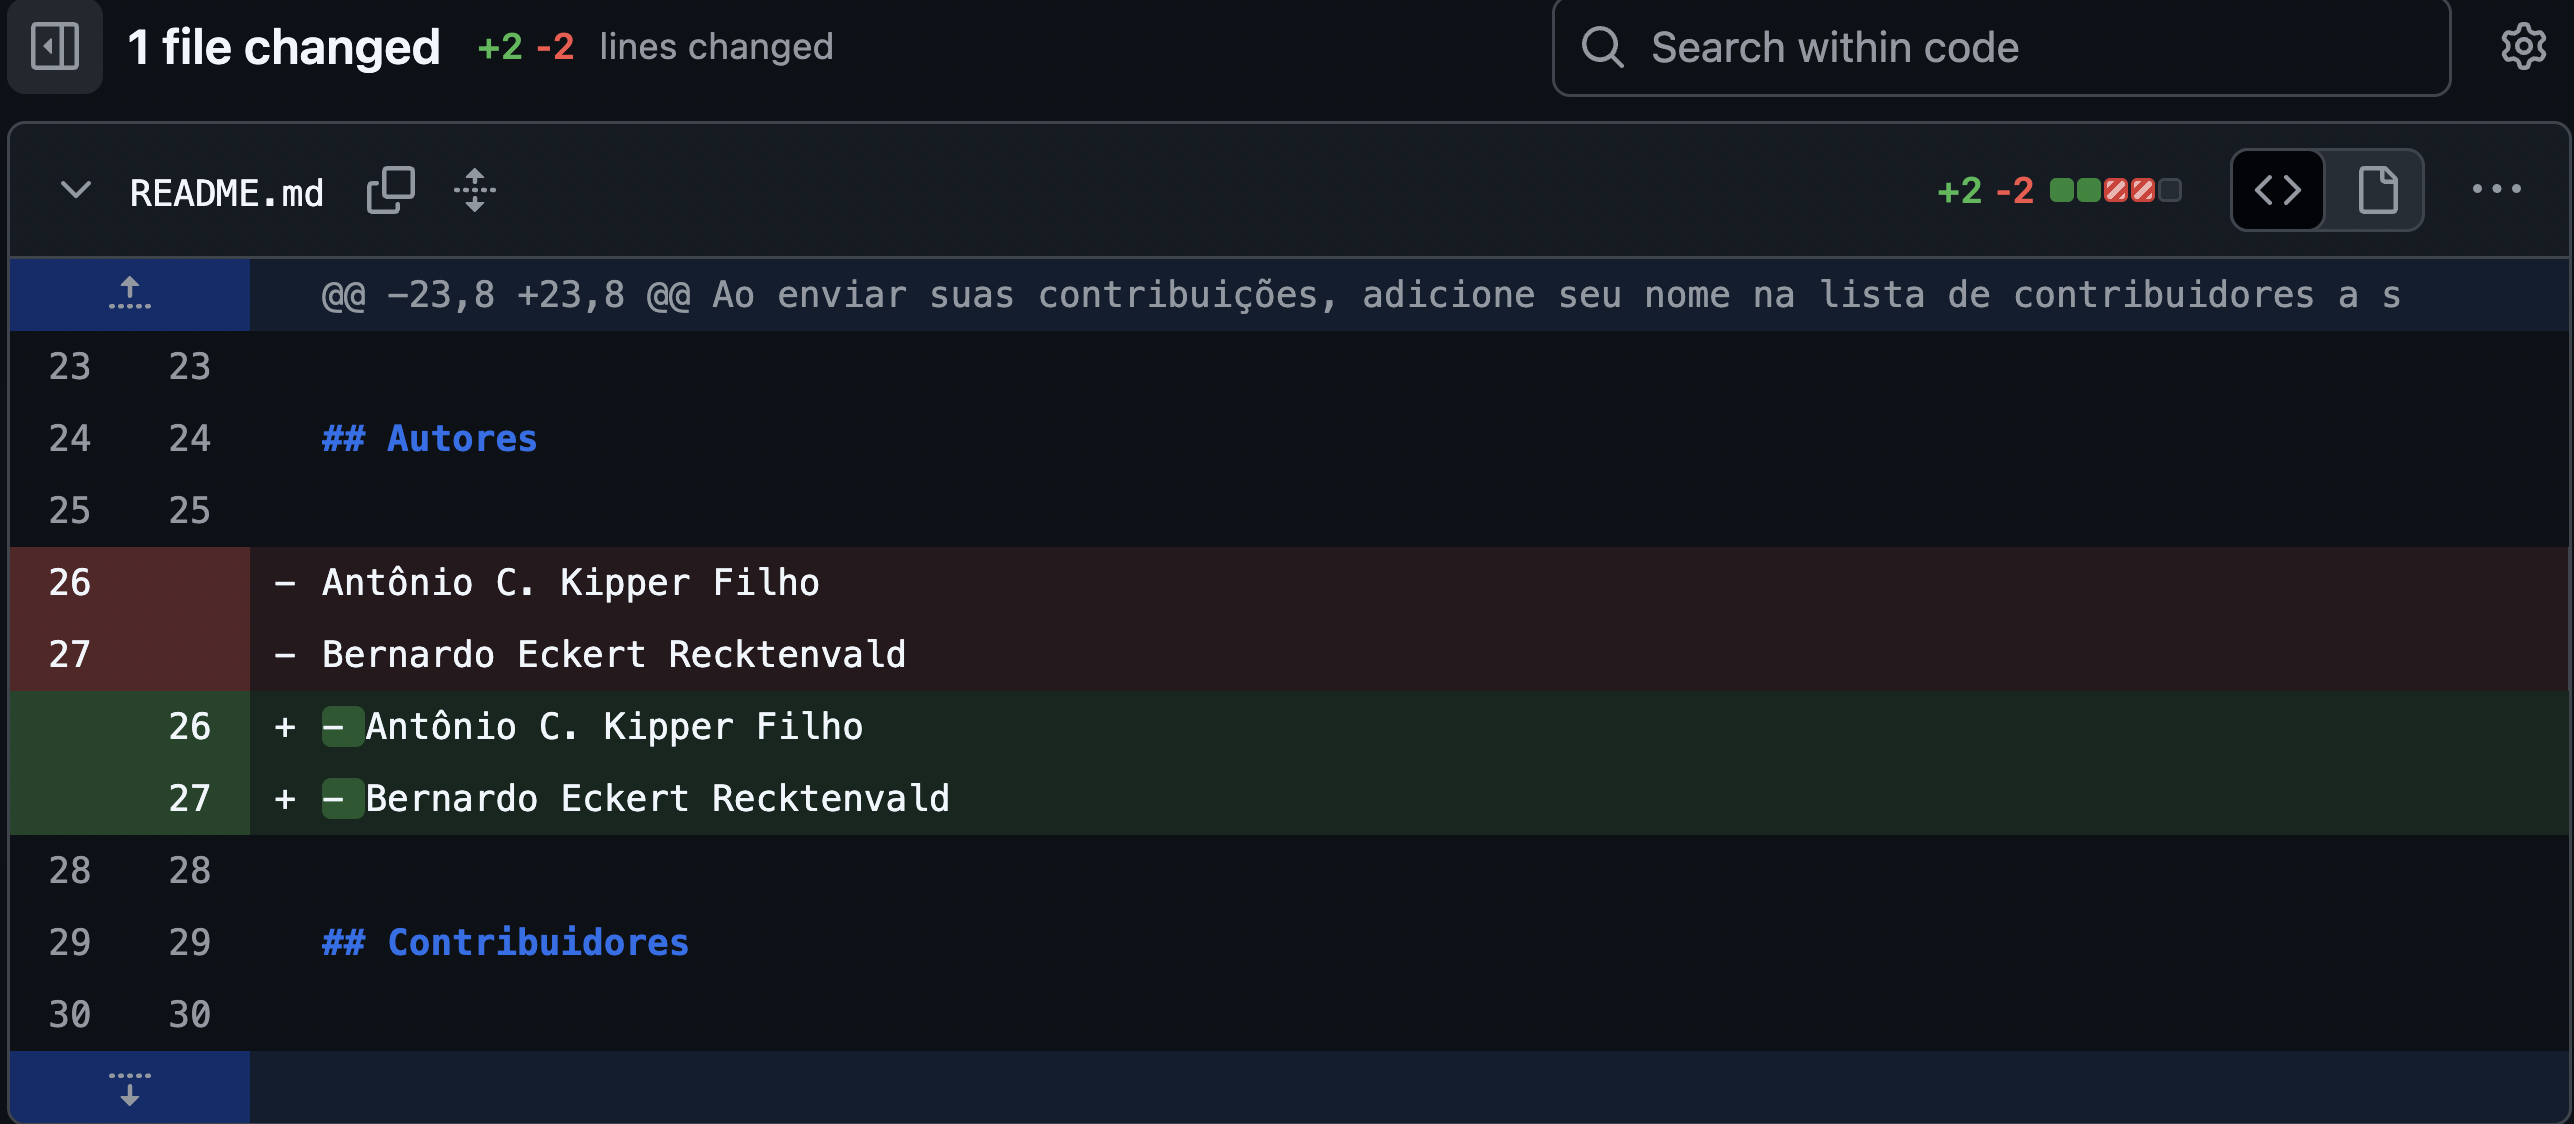
\includegraphics[width=0.6\textwidth]{imgs/tutorial_contribuicao/README_modif.png}
        \caption{Modificações no README - adicionar "-" antes de cada nome para exibição correta como item.}
        \label{fig:README_modif}
    \end{figure}

        \item O resultado esperado é este:

        \begin{figure}[H]
        \centering
        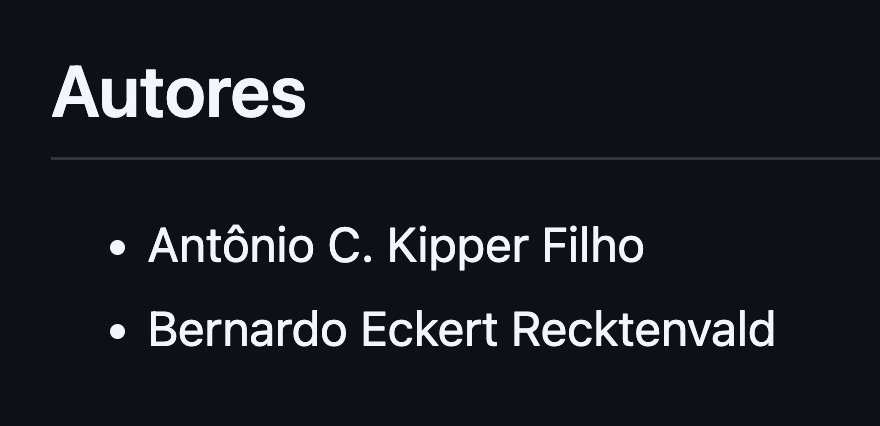
\includegraphics[width=0.6\textwidth]{imgs/tutorial_contribuicao/README_depois_modif.png}
        \caption{README corrigido.}
        \label{fig:README_depois_modif}
    \end{figure}

        \item Adicione, faça commit e envie para seu repositório:
        \begin{lstlisting}[style=shellstyle]
git add .
git commit -m "Descreva sua contribuição"
git push origin minha-contribuicao
        \end{lstlisting}

        \item Na sequência, abra novamente o seu repositório no Github e navegue para a branch de contribuições:

         \begin{figure}[H]
        \centering
        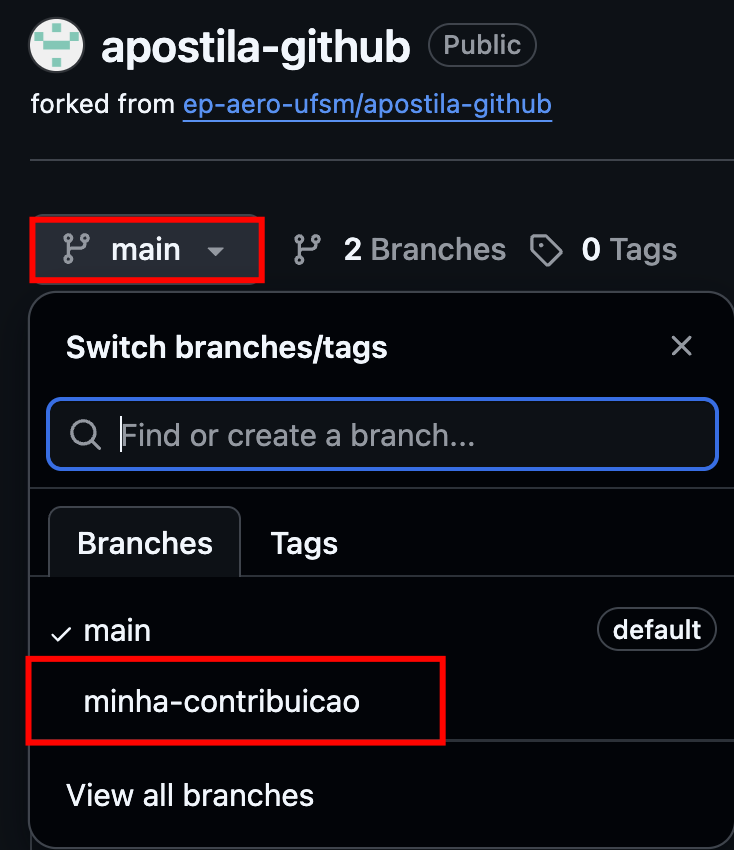
\includegraphics[width=0.6\textwidth]{imgs/tutorial_contribuicao/navegando_branch.png}
        \caption{Navegue para a branch minha-contribuicao.}
        \label{fig:navegando_branch}
    \end{figure}

        \item Abra um Pull Request no repositório original da EP Aero pelo Github. Para fazer isso, siga os passos a seguir:

    \begin{figure}[H]
        \centering
        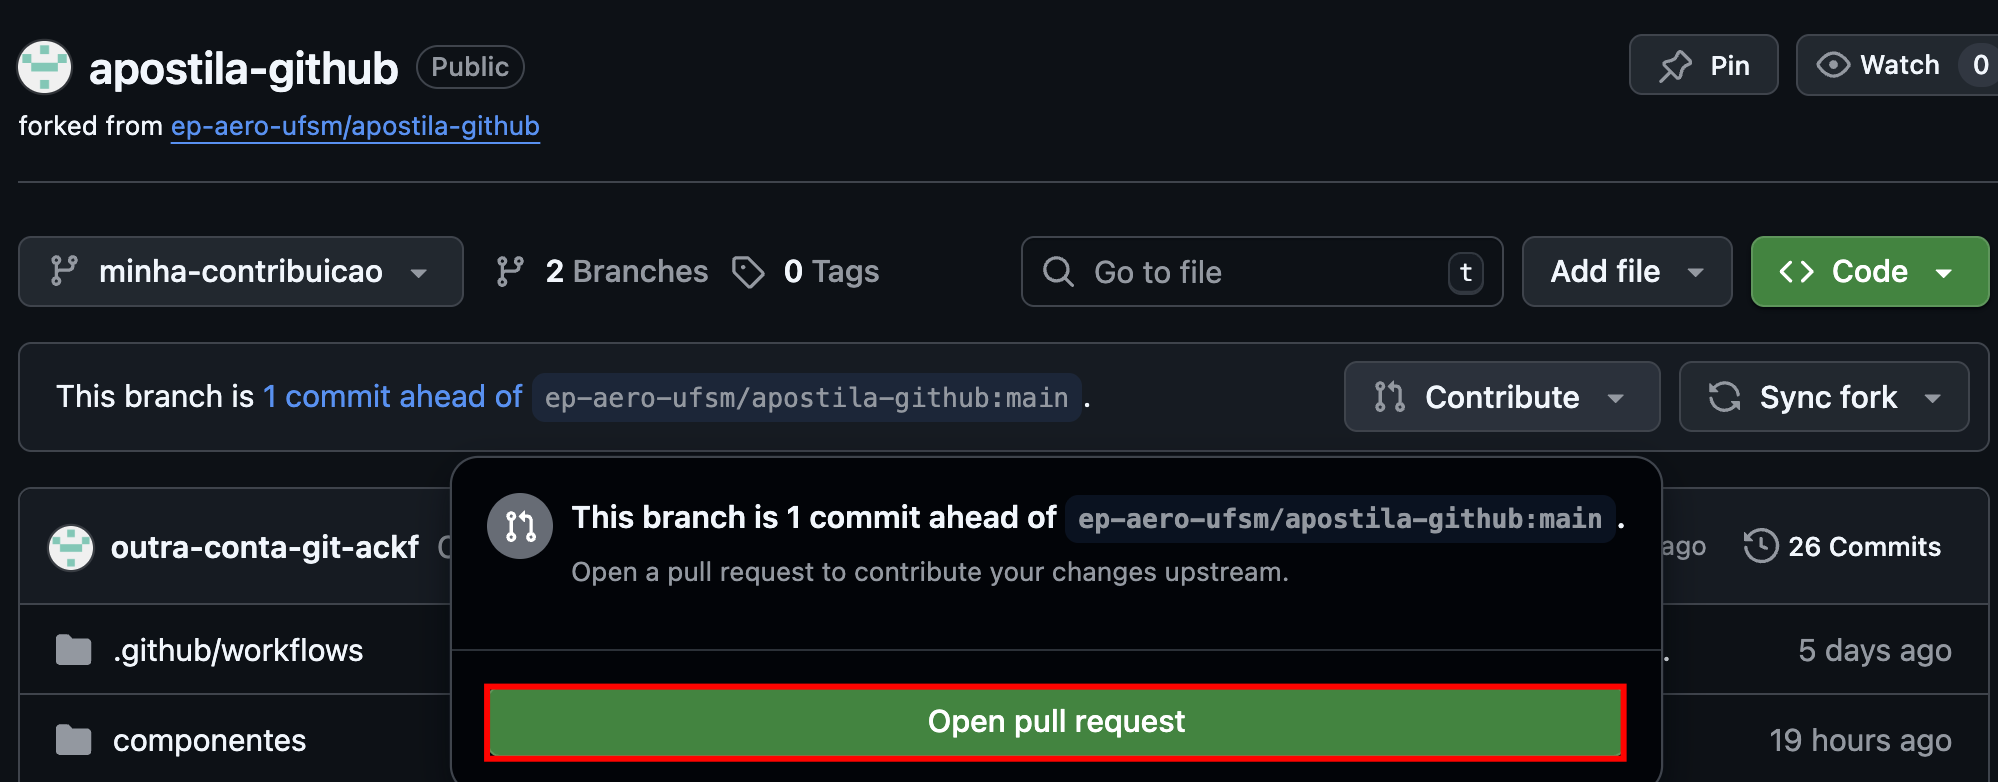
\includegraphics[width=0.6\textwidth]{imgs/tutorial_contribuicao/abrir_pull_request.png}
        \caption{Abra um pull request na sua branch.}
        \label{fig:abrir_pr}
    \end{figure}

    \begin{figure}[H]
        \centering
        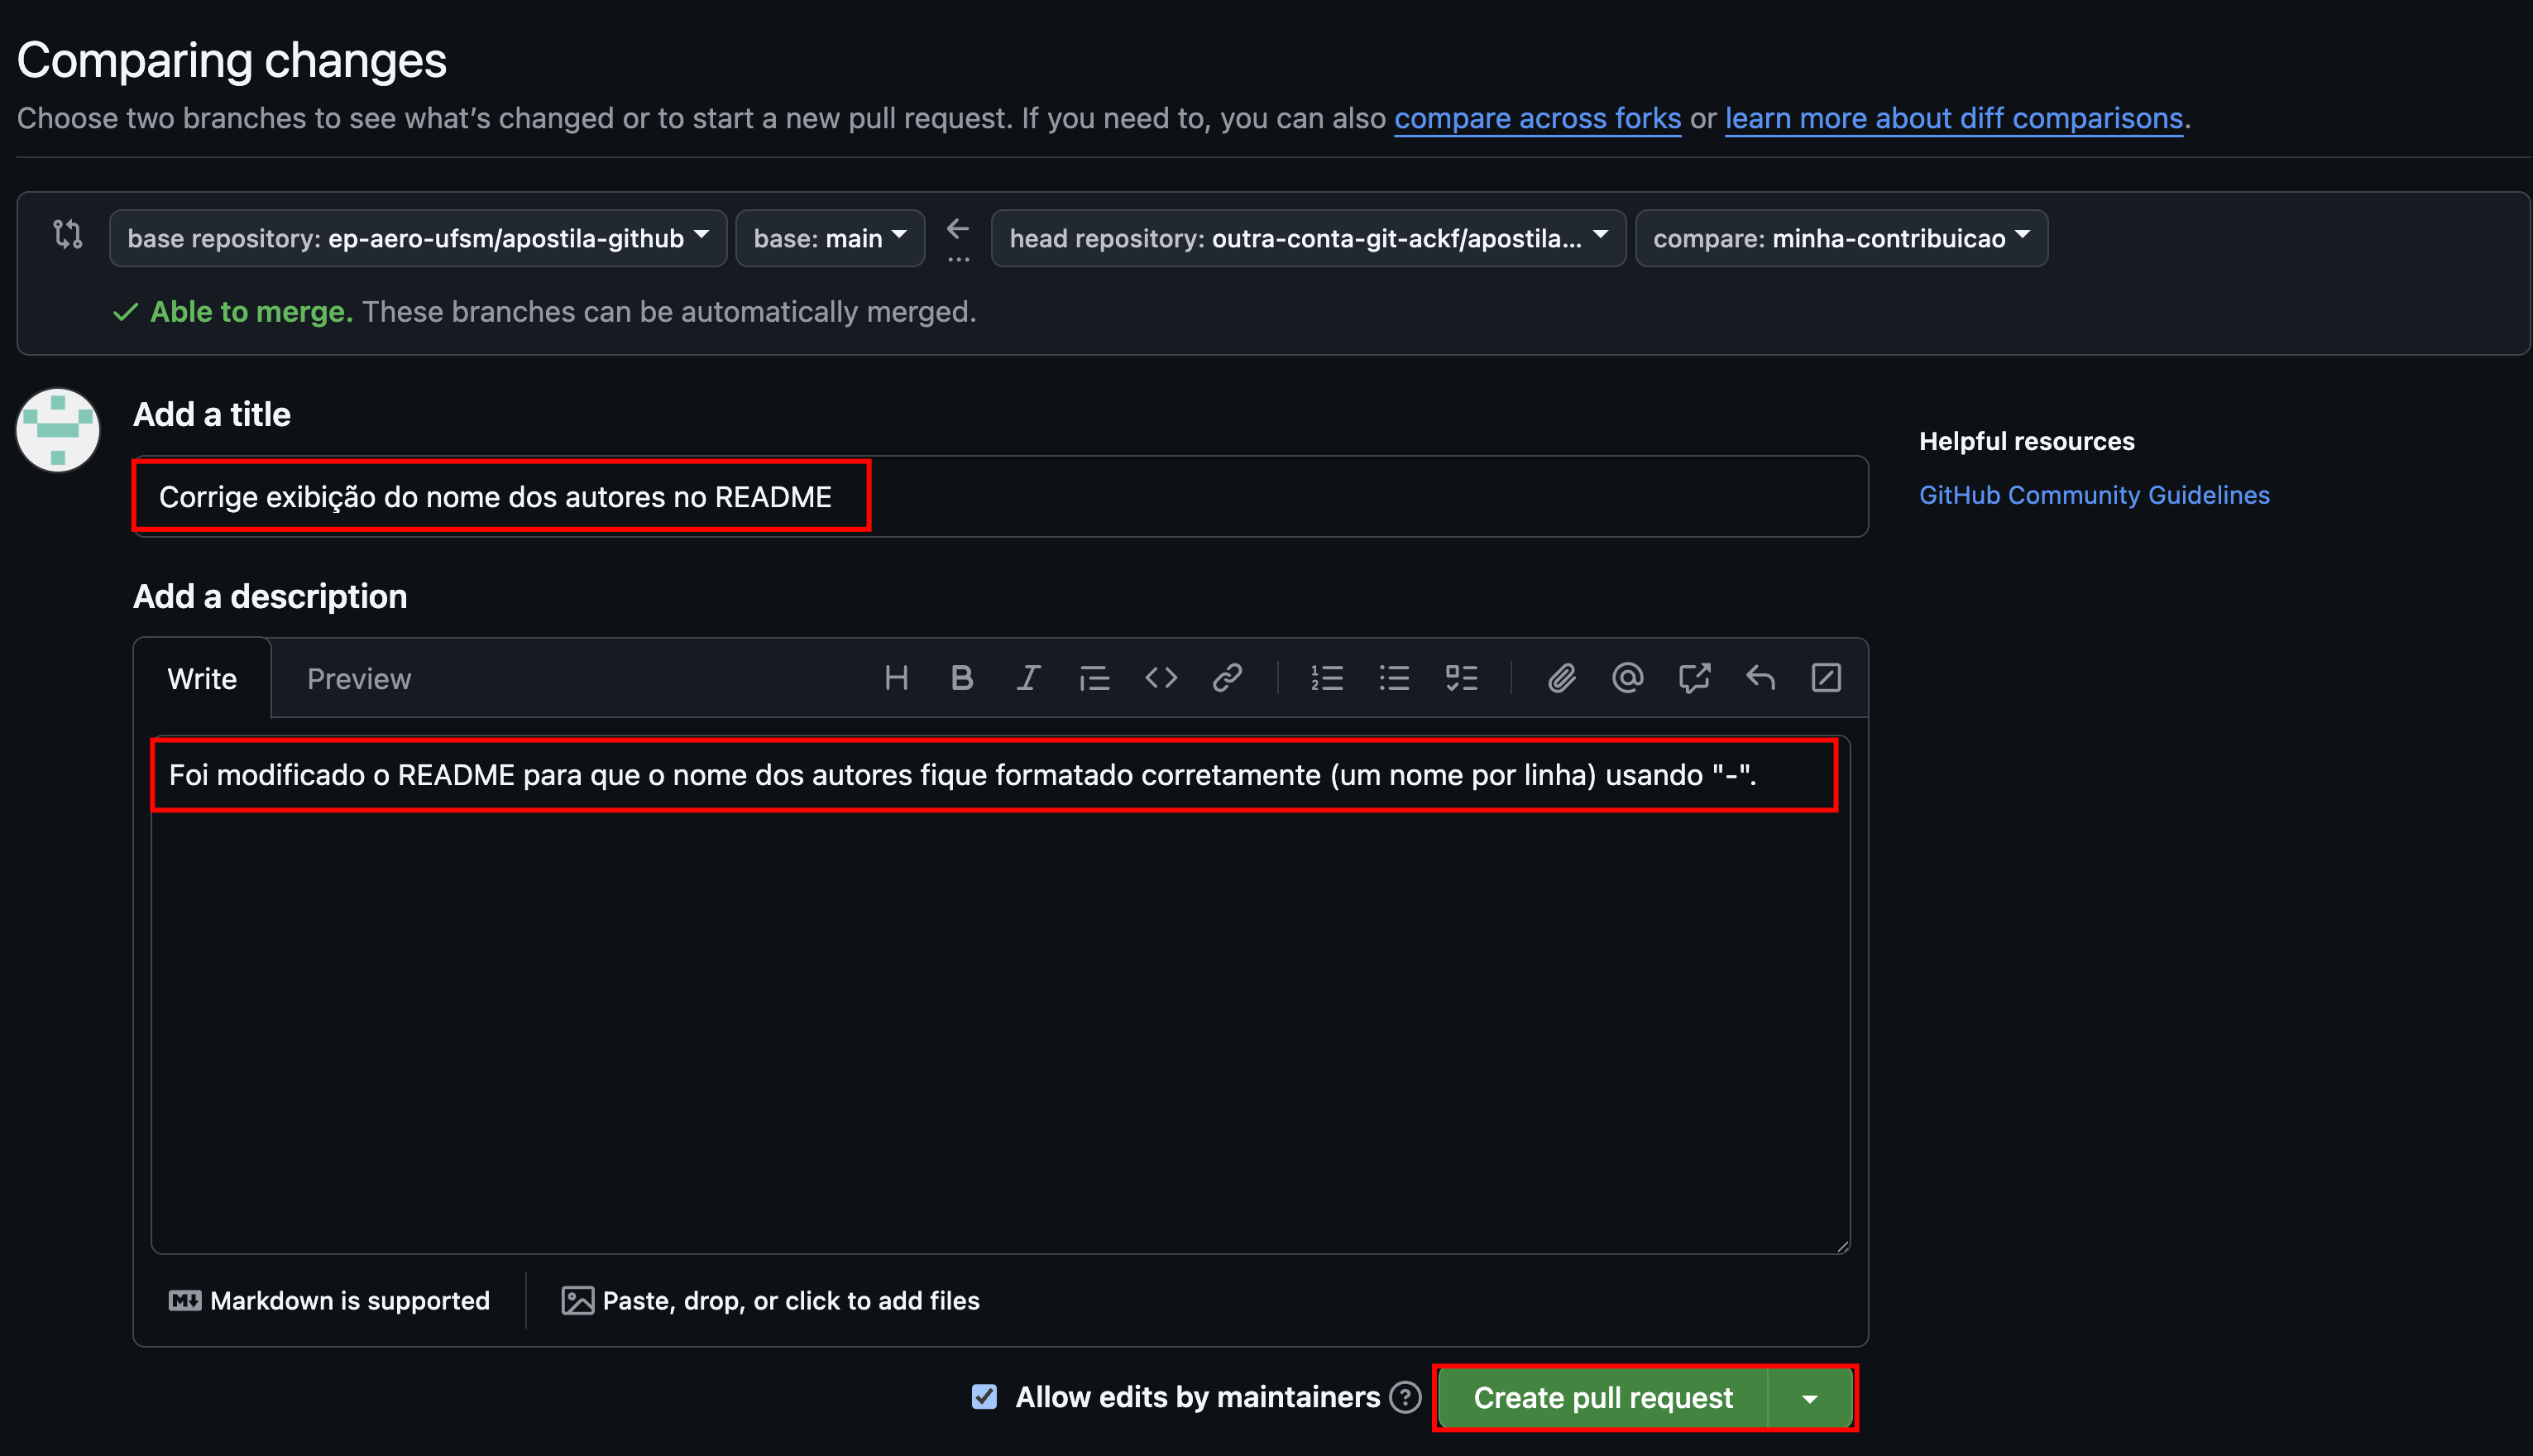
\includegraphics[width=0.6\textwidth]{imgs/tutorial_contribuicao/configurando_pull_request.png}
        \caption{Descreva o pull request. Use um título e uma descrição concisa, mas precisa.}
        \label{fig:configurar_pr}
    \end{figure}

    \item Na sequência, um dos mantedores do repositório da EP Aero UFSM irá analisar seu pull request, e poderá ou aceitá-lo diretamente, ou rejeitá-lo pedindo algum tipo de correção. Caso esse seja o caso, você receberá uma mensagem como esta no seu pull request:

    \begin{figure}[H]
        \centering
        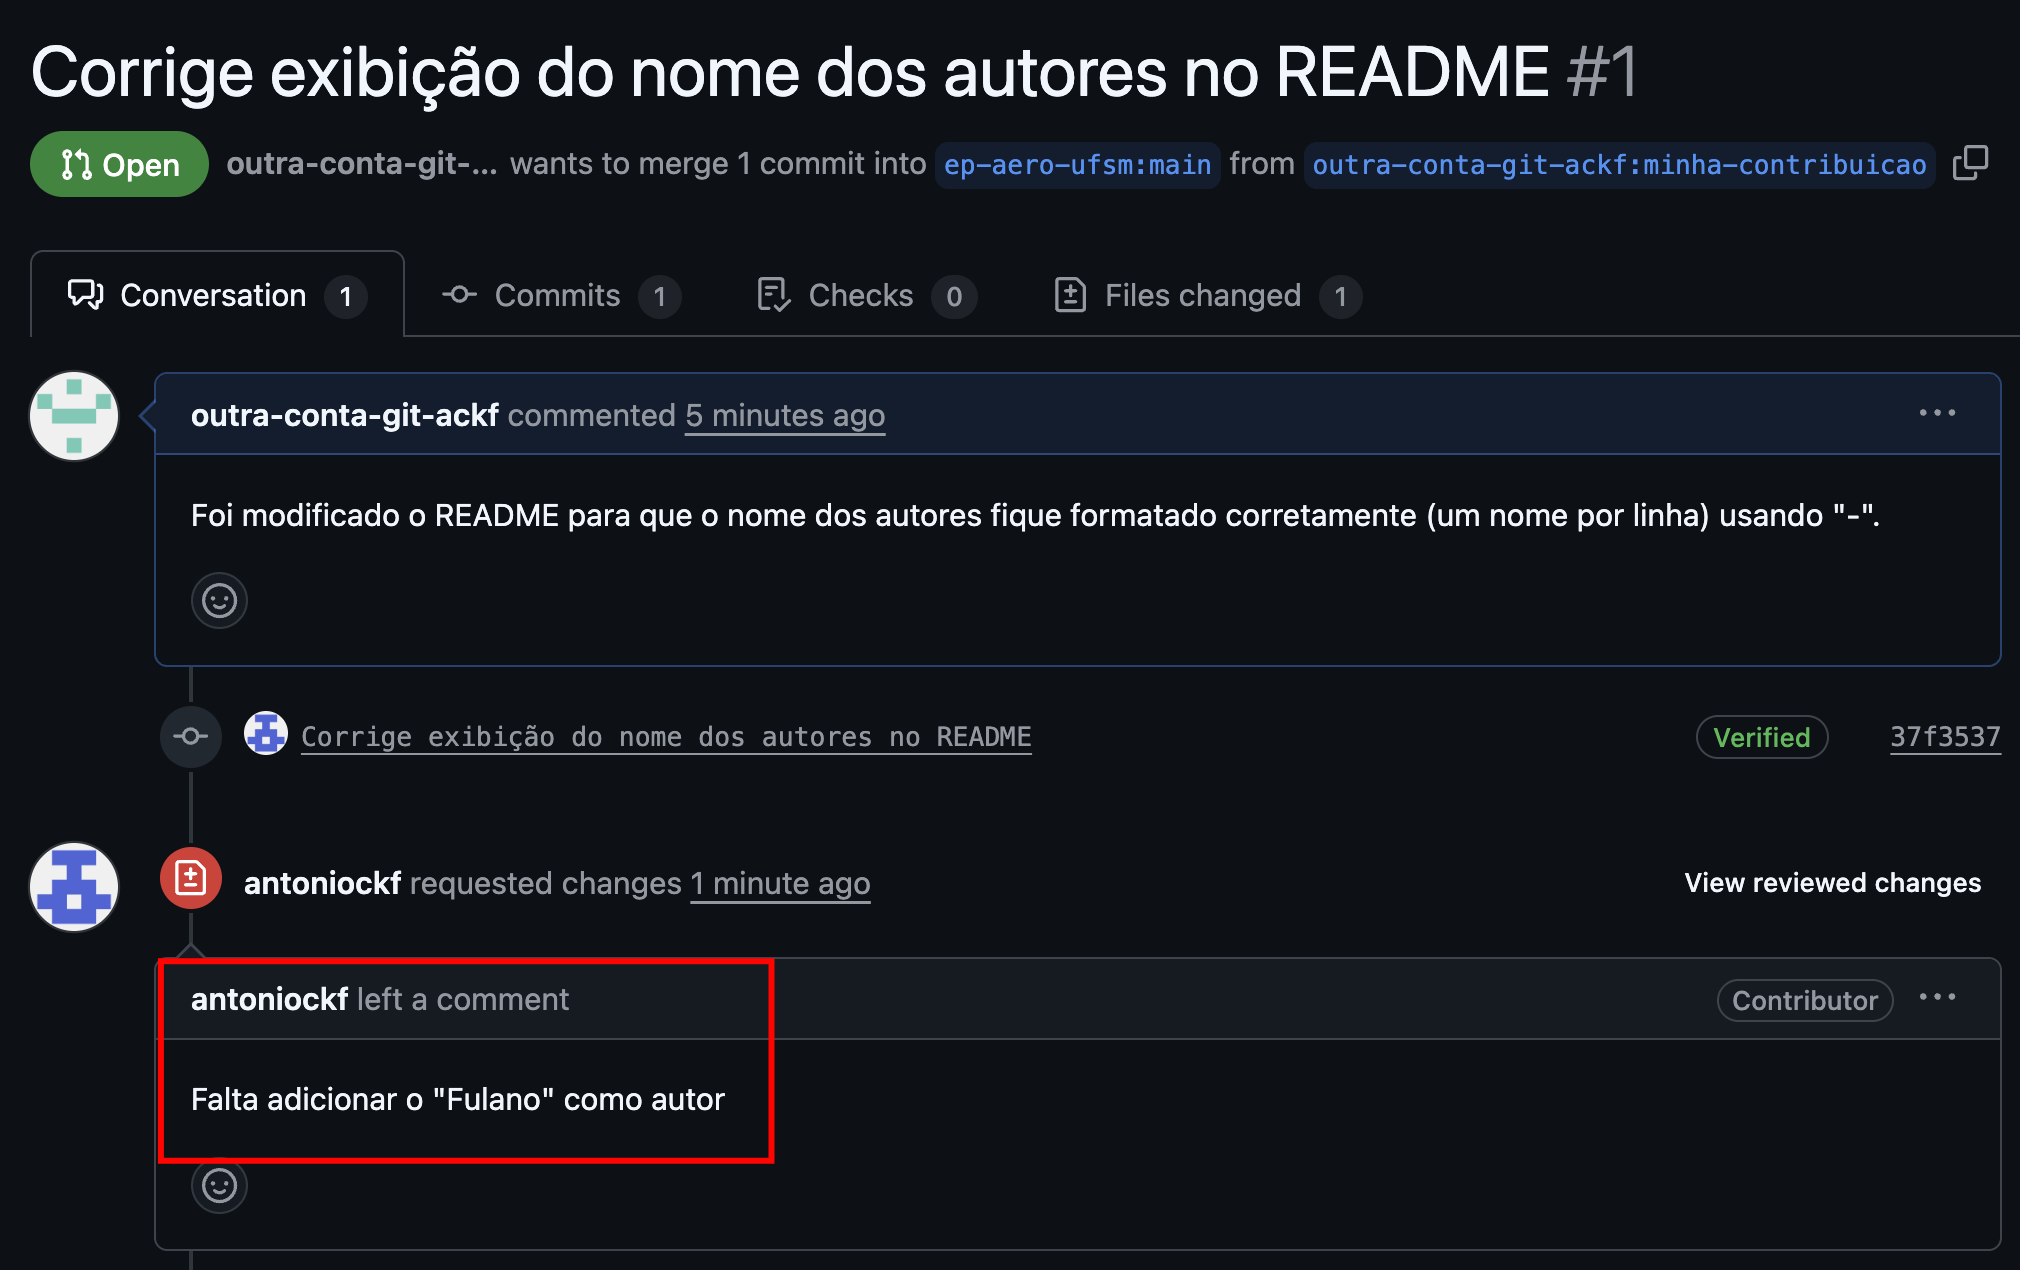
\includegraphics[width=0.6\textwidth]{imgs/tutorial_contribuicao/pr_rejeitado.png}
        \caption{Pull request rejeitado - os mantedores solicitam modificações.}
        \label{fig:pr_rejeitado}
    \end{figure}

    \item Você deve então fazer um novo commit na sua branch com as correções pedidas. O novo commit aparecerá automaticamente no Pull Request que você havia enviado antes:

    \begin{figure}[H]
        \centering
        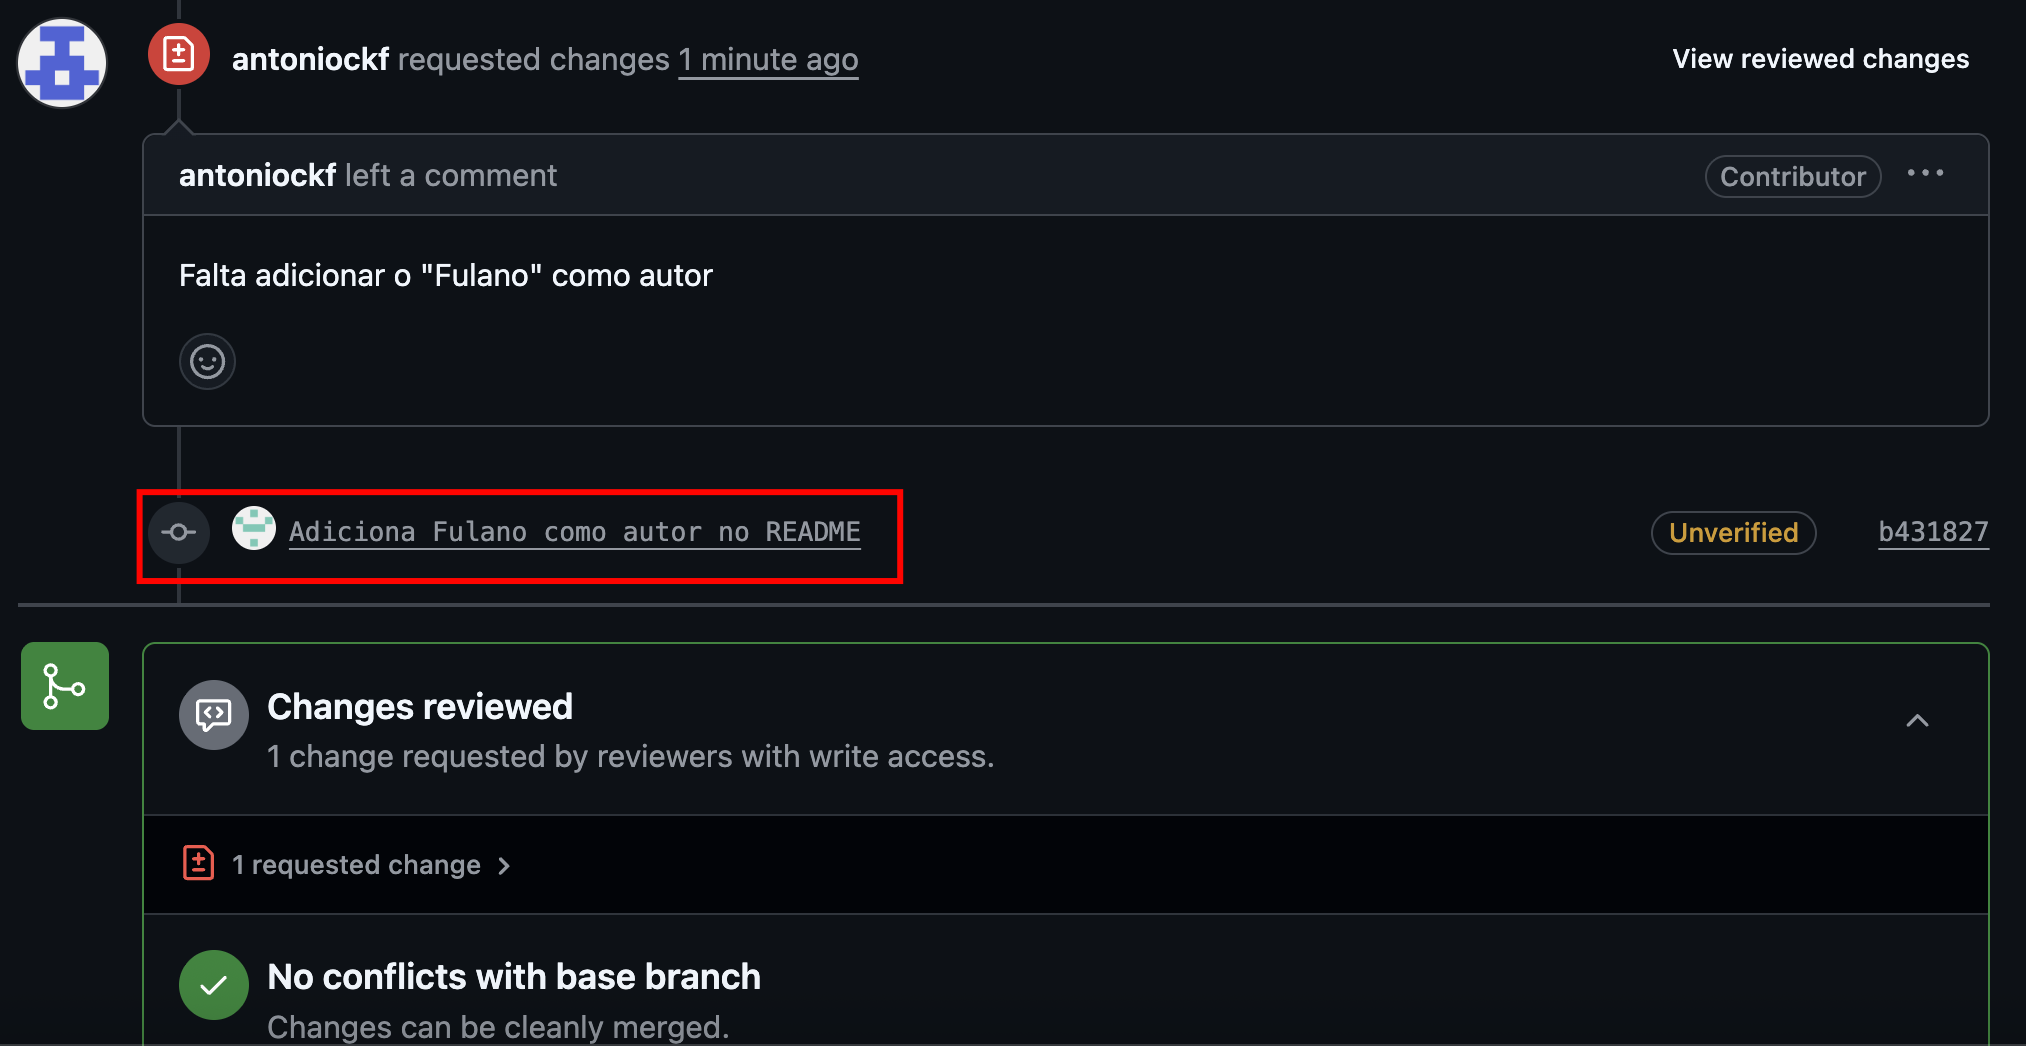
\includegraphics[width=0.6\textwidth]{imgs/tutorial_contribuicao/replica_pr.png}
        \caption{Mudança no PR após solicitação de correção.}
        \label{fig:replica_pr}
    \end{figure}

    \item Quando o PR for aceito, ele aparecerá na história de commits da branch principal do repositório da EP Aero: 

    \begin{figure}[H]
        \centering
        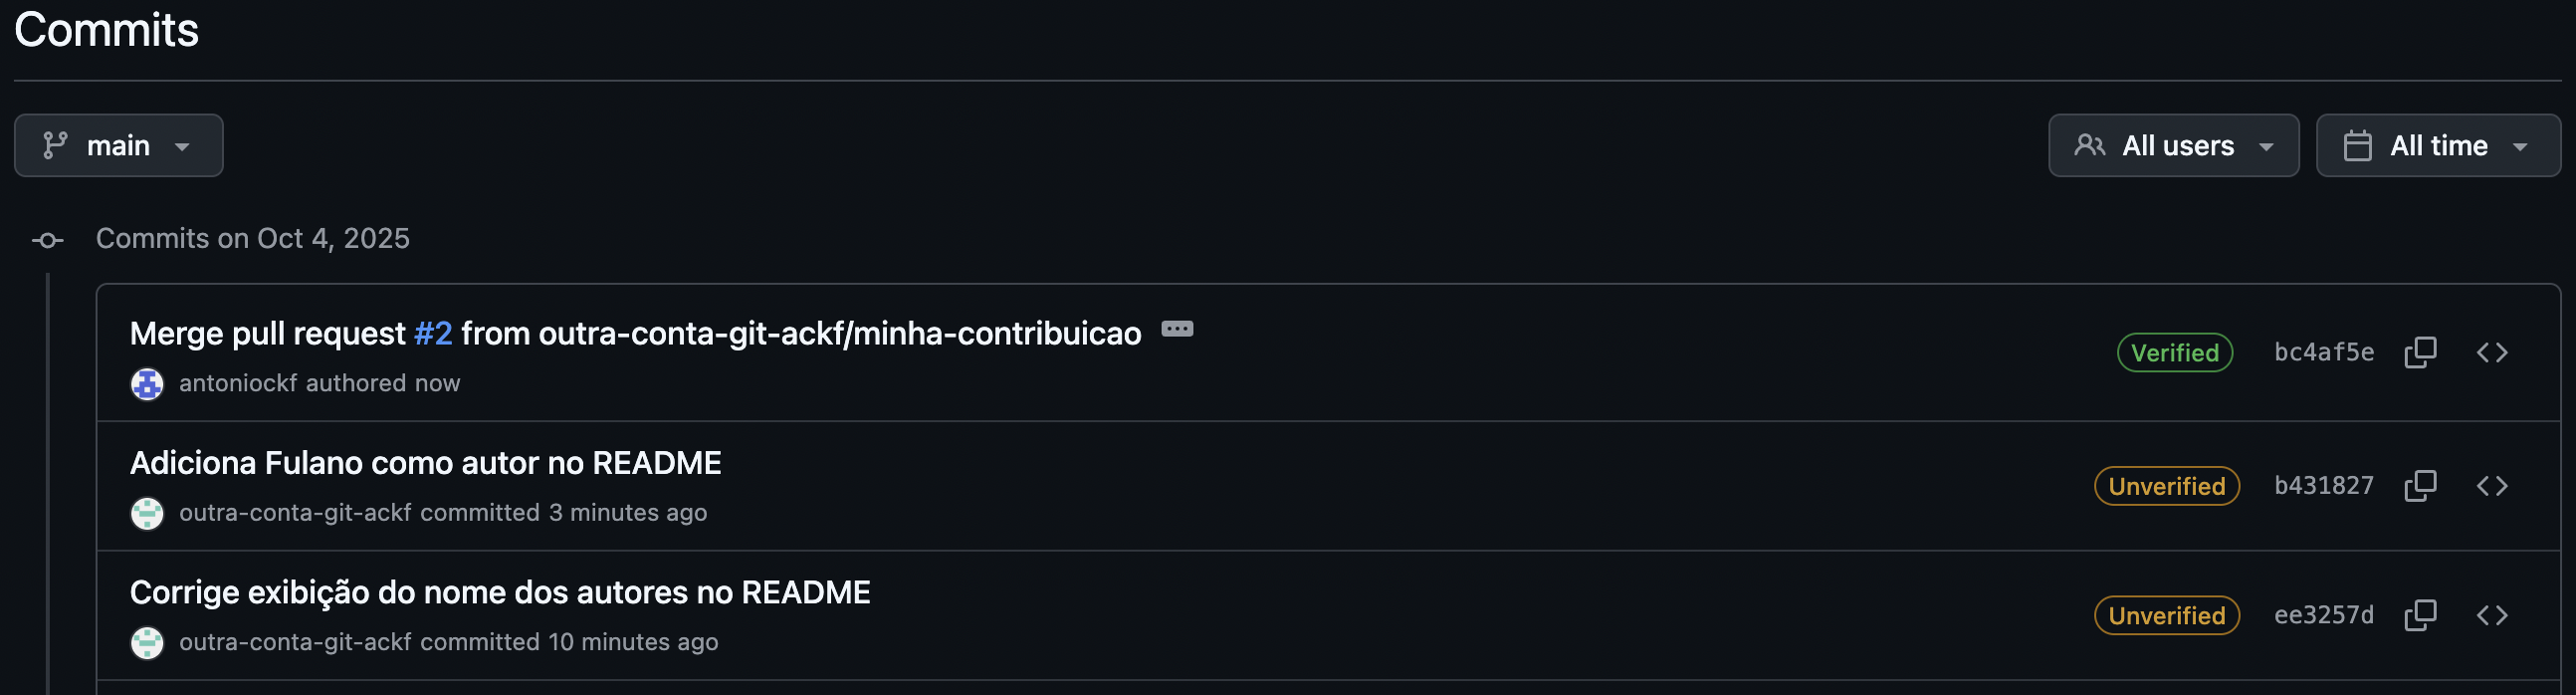
\includegraphics[width=0.6\textwidth]{imgs/tutorial_contribuicao/resultado_pr.png}
        \caption{Resultado final após merge do PR.}
        \label{fig:resultado_pr}
    \end{figure}
\end{itemize}

    \newpage
\section{Recursos e Referências}

Para aprofundar seus conhecimentos em Git e trabalho colaborativo, é importante consultar materiais de referência e recursos oficiais. Abaixo estão algumas recomendações úteis para estudo e consulta durante o desenvolvimento de projetos.

\subsection{Documentação Oficial do Git}

A documentação oficial do Git é completa e detalhada, abordando desde conceitos básicos até comandos avançados. Recomenda-se a leitura para esclarecer dúvidas e explorar funcionalidades adicionais.

\begin{itemize}
    \item Site oficial: \url{https://git-scm.com/doc}
    \item Livro gratuito: \url{https://git-scm.com/book/en/v2}
\end{itemize}

\subsection{GitHub Learning Lab}

O GitHub Learning Lab oferece cursos interativos gratuitos sobre Git, GitHub e colaboração em projetos. Os exercícios são práticos e guiados, ideais para iniciantes e para quem deseja aprimorar suas habilidades.


%% ber - o link daqui estava quebrado
\begin{itemize}
    \item Acesse: 
\end{itemize}

\subsection{Cheat Sheets Recomendados}

Cheat sheets são resumos práticos dos principais comandos e fluxos de trabalho do Git, úteis para consulta rápida durante o desenvolvimento.

\begin{itemize}
    \item Git Cheat Sheet oficial: \url{https://education.github.com/git-cheat-sheet-education.pdf}
    \item GitHub Git Cheat Sheet: \url{https://github.github.com/training-kit/downloads/github-git-cheat-sheet.pdf}
    \item Atlassian Git Cheat Sheet: \url{https://www.atlassian.com/git/tutorials/atlassian-git-cheatsheet}
\end{itemize}

Esses recursos complementam o conteúdo da apostila e ajudam a resolver dúvidas, explorar novas funcionalidades e aprimorar o uso do Git em projetos acadêmicos

    
    
\end{document}
